\section{Kondensierte Materie 2}
\subsection{Dielektrische und optische Eigenschaften}
\noindent\textbf{1. Welcher Zusammenhang besteht zwischen der dielektrischen Funktion und den optischen Eigenschaften eines Festkörpers?}\\
\begin{addmargin}[25pt]{0pt}
Die dielektrische Funktion $\varepsilon$ kann aufgeteilt werden in einen Realteil $\varepsilon'$ und einen Imaginärteil $\varepsilon''$. Der direkte Zusammenhang mit den optischen Eigenschaften ist, dass das Quadrat des komplexen Brechungsindexes $n = n' + i\kappa$ gleich der dielektrischen Funktion entspricht:
\begin{equation}\label{eq:epsilon_n}
    \varepsilon' + i\varepsilon'' = (n' + i\kappa)^2
\end{equation}
oder ausmultipliziert:
\begin{align}
    \varepsilon' &= n'^2 -\kappa^2\\
    \varepsilon'' &= 2n'\kappa
\end{align}
Aus dieser Eigenschaft folgt direkt die Verbindung von $\varepsilon$ mit dem Reflexionsgrad $R$:
\begin{equation}\label{eq:epsilon_R}
    R = \left| \frac{\sqrt{\varepsilon} - 1}{\sqrt{\varepsilon} + 1}\right|^2
\end{equation}
\end{addmargin}

\noindent\textbf{2. Welches elektrische Feld wirkt lokal an der Position eines Atoms in einem polarisierbaren Festkörper, der sich in einem homogenen äußeren elektrischen Feld befindet?}\\
\begin{addmargin}[25pt]{0pt}
An dieser Position wirkt sowohl das äußere elektrische Feld $\mathbf{E}_a$ als auch ein elektrisches Feld aufgrund der im Festkörper relativ nahen Nachbaratome. Die Summe dieser Beiträge heißt lokales Feld $\mathbf{E}_{lok}$. In genauerer Betrachtung weißt das lokale Feld 4 Komponenten auf. Eine dieser Komponenten ist das äußere Feld $\mathbf{E}_a$ selbst. Eine zweite Komponente ist das Depolarisationsfeld $\mathbf{E}_D$, das entsteht ,da im gesamten Festkörper die Atome polarisiert werden und so an der Oberfläche des Körpers eine induzierte Oberflächenladung erzeugt wird. Das Feld dieser Ladung wirkt dem äußeren Feld entgegen. Ein dritter Beitrag ist das Lorentzfeld $\mathbf{E}_L$. Dieses entsteht da jedes Atom, also insbesondere auch die nah am Betrachtungsort des lokalen Feldes, polarisiert sind. Durch diese Dipole entsteht das Lorentzfeld $\mathbf{E}_L = \frac{1}{3\varepsilon_0}\mathbf{P}$. $\mathbf{P}$ ist die Polarisierung des Körpers. Der letzte Beitrag zum lokalen Feld ist die direkte Wirkung von benachbarten Atomen. Diese werden ohne Polarisierung betrachtet. Dieser Teil ist, bei Summation über alle Nachbarn, aus Symmetriegründen ungefähr null. \\
\end{addmargin}

\noindent\textbf{3. Wie können wir Festkörper hinsichtlich ihrer Reaktion auf äußere elektrische Felder klassifizieren?}\\
\begin{addmargin}[25pt]{0pt}
Man kann Festkörper einteilen in dielektrische, paraelektrische und ferro- bzw. antiferroelektrische Festkörper. Dielektrische Festkörper bilden unter dem Einfluss externer Felder im atomaren Bereich Dipole aus. Diese Dipole entstehen entweder durch Verschiebung der Elektronenwolke um den Atomkern oder durch Verschiebung der Ionen relativ zueinander. In paraelektrischen Materialien treten auch ohne äußeres Feld bereits Dipole auf, diese sind allerdings ungeordnet, wodurch kein makroskopisches elektrisches Feld messbar ist. Sobald ein äußeres elektrisches Feld angelegt wird orientieren sich diese Dipole alle in eine Richtung und man misst ein elektrisches Feld aufgrund dieser \textit{Orientierungspolarisation}. In ferroelektrischen Materialien tritt auch ohne äußeres Feld eine Polarisation auf. \\
\end{addmargin}

\noindent\textbf{4. Was beschreibt das Lorentz'sche Oszillatormodell?}\\
\begin{addmargin}[25pt]{0pt}
    Das Lorentz'sche Oszillatormodell wird angenommen, dass die an einem Atomkern gebundenen Elektronen sich so verhalten, als wären sie mit einer Feder am Atomkern befestigt. Durch äußere Bestrahlung mit Licht, dessen $\mathbf{E}$-Feld Komponente harmonisch oszilliert, wird das Elektron zum Schwingen angeregt und aus der Auslenkung kann die Polarisierbarkeit bestimmen werden.  \\
\end{addmargin}

\noindent\textbf{5. Was ist ein Polariton?}\\
\begin{addmargin}[25pt]{0pt}
Das Polariton ist ein Quasiteilchen, welches entsteht wenn ein elektromagnetisches Feld an ein transversal-optisches-Phonon koppelt. Bei starker Kopplung zwischen Phonon und Photon kann man den Prozess nicht mehr mit der Störungstheorie beschreiben. In diesem Fall  wird das Polariton benötigt um die Anregung zu beschreiben. In ionischen Kristallen ruft das Photon eine lokale Polarisation hervor, welche gleichbedeutend mit einer Gitterverzerrung ist. Diese Gitterverzerrung wird durch das Polariton beschrieben. Polaritonen entstehen in ionischen Kristallen.\\
\end{addmargin}

\noindent\textbf{6. Wie verhält sich die Dispersionsrelation eines Polaritons für $\omega < \omega_t$ und $\omega > \omega_l$?}\\
\begin{addmargin}[25pt]{0pt}
Für ganz kleine Frequenzen kann der Kristall aufgrund der geringen Energie des Lichts nicht zu Schwingungen angeregt werden, die Dispersionsrelation verhält sich also wie die von Photonen. Mit steigender Frequenz (bis zu $\omega_t$) werden immer mehr Gitterschwingungen angeregt bis sich die Polaritonen bei $\omega = \omega_t$ wie transversal-optische Phononen verhalten. Für Frequenzen $\omega >\omega_l$ werden erst nur Schwingungen angeregt also verhalten sich die Polaritonen wie Phononen. Bei noch höheren Frequenzen verhalten sie sich wieder wie Photonen weil das Licht so hochfrequent ist, dass keine Schwingungen angeregt werden können.   \\
\end{addmargin}

\noindent\textbf{7. Was passiert im Bereich $\omega_t < \omega < \omega_l$?}\\
\begin{addmargin}[25pt]{0pt}
Licht mit dieser Frequenz kann sich im Körper nicht ausbreiten, das Licht wird totalreflektiert. Dadurch gibt es im Festkörper weder Photonen noch Gitterschwingungen, wodurch auch keine Polaritonen entstehen.\\
\end{addmargin}

\noindent\textbf{8. Was sind Plasmonen?}\\
\begin{addmargin}[25pt]{0pt}
Das Plasmon ist das Quasiteilchen der Plasmaschwingung. Es beschreibt die Schwingung in einem Plasma, wie zum Beispiel die Oszillationen der Dichte in einem freien Elektronengas. Plasmonen können, ähnlich wie Phononen, an Photonen koppeln, dabei entsteht dann ein Plasmon-Polariton. \\
\end{addmargin}



\subsection{Halbleiter}
\subsubsection{Kurzfragen basierend auf den Übungsblättern von Professor Back}
\noindent\textbf{1. Wie kann man aus der Formel für die Stromdichte an einem pn-Übergang die Sperrrichtung und die Durchlassrichtung erkennen?}\\
\begin{addmargin}[25pt]{0pt}
 Für die Stromdichte an einem pn-Übergang gilt:
 \begin{equation}\label{eq:Strom_pn_transition}
      j(U) \propto \exp(\frac{eU}{k_BT}) -1
 \end{equation}
 Man kann anhand von Gleichung \ref{eq:Strom_pn_transition} erkennen, dass bei $U<0$ die Exponentialfunktion eine Wert zwischen null und eins annimmt, die Stromdichte ist somit für jeden Wert von $U$ relativ klein. Im Fall von $U>0$ also der Durchlassrichtung wird der Strom sehr schnell sehr stark ansteigen.   
 \end{addmargin}


\noindent\textbf{2. Wie sieht die Strom-Spannungskennlinie für einen pn-Übergang aus?}\\
\begin{addmargin}[25pt]{0pt}
\begin{figure}[h]
    \centering
    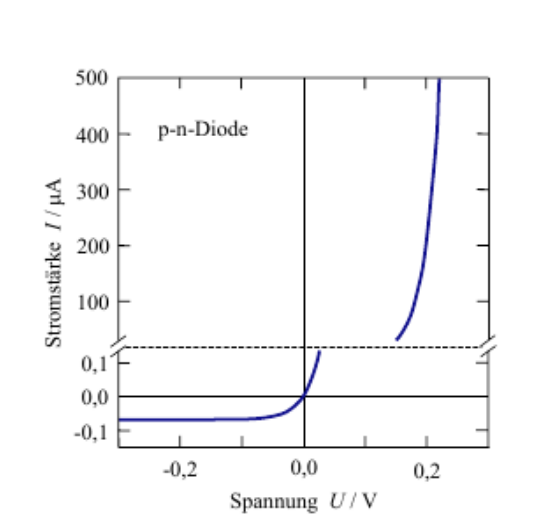
\includegraphics[width = 0.8\textwidth]{images/KM2/pn_transition_Strom_Spannung.png}
    \caption{Verlauf des Stroms in Abhängigkeit der Spnnung am pn-Übergang}
    \label{fig:pn_transition_Strom_Spannung}
\end{figure} 
Die Strom-Spannungskennlinie ist in Abbildung \ref{fig:pn_transition_Strom_Spannung} dargestellt. Man erkennt, dass in der Durchlassrichtung, also $U>0$ der Stromfluss um mehrere Größenordnungen höher ist als in der Sperrrichtung.\\
 \end{addmargin}

\noindent\textbf{3. Wie sieht das Banddiagramm für eine Schottky-Barriere aus für den Fall, dass Metall und Halbleiter voneinander getrennt sind und für den Fall dass sie in Kontakt stehen?}\\
\begin{addmargin}[25pt]{0pt}
    \begin{figure}[h]
        \centering
        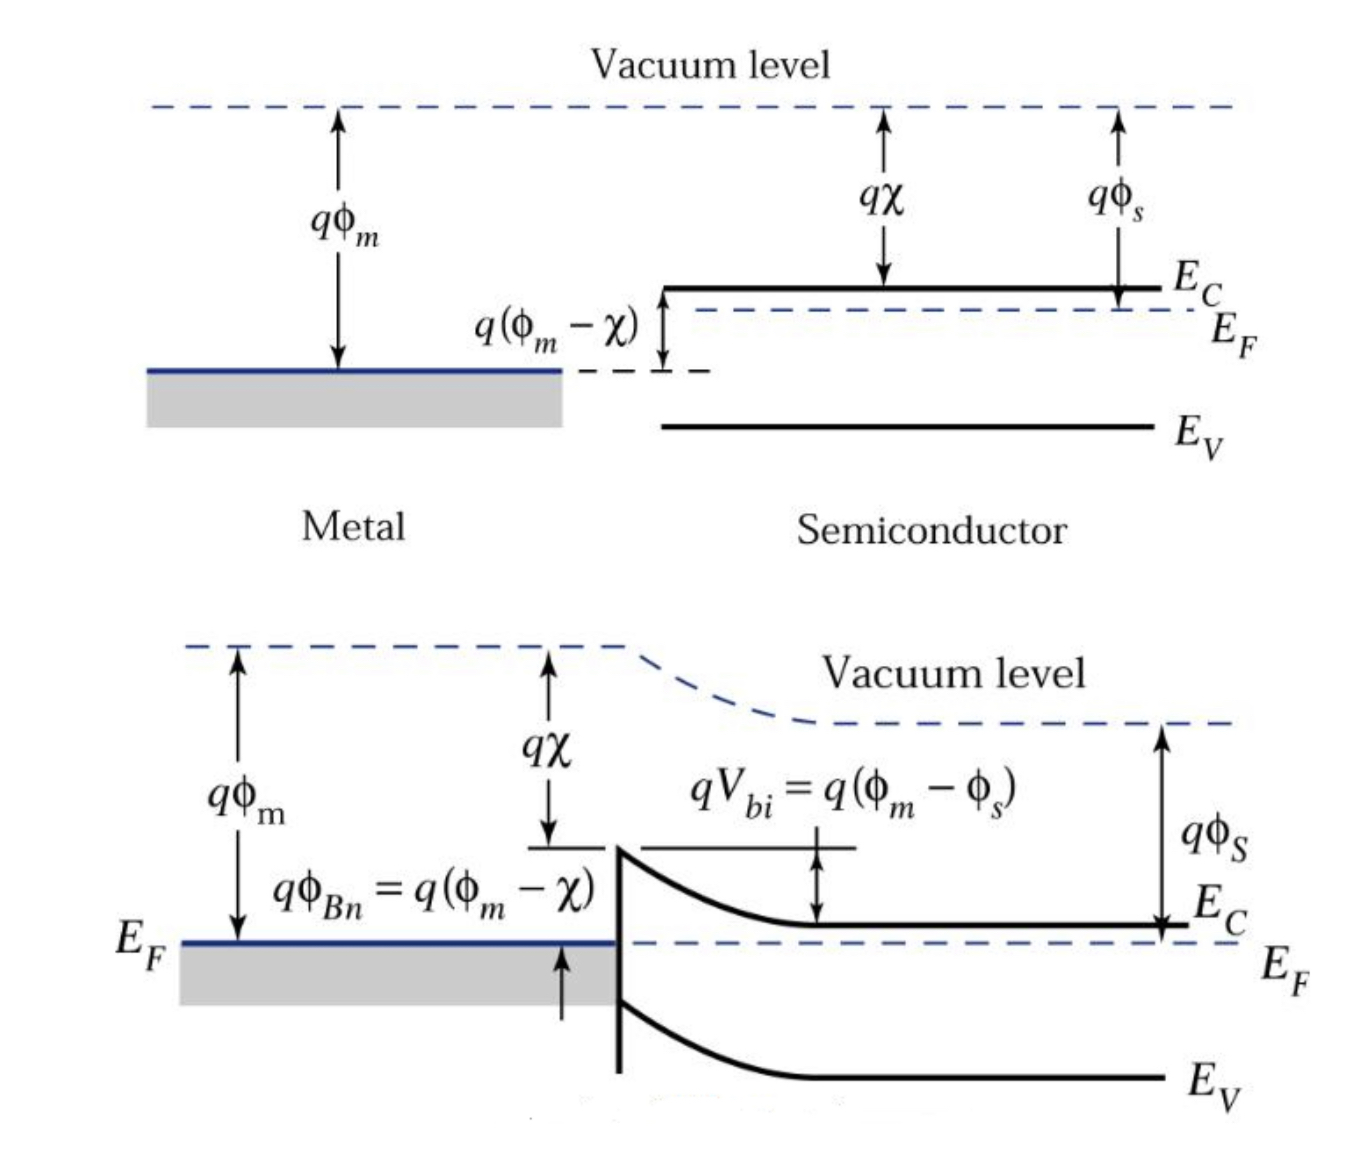
\includegraphics[width = 0.8\textwidth]{images/KM2/Schottky-Barriere.jpeg}
        \caption{Banddiagramm Schottky-Barriere}
        \label{fig:Schottky-Barriere}
    \end{figure}
    Die Banddiagramme sind in Abbildung \ref{fig:Schottky-Barriere} dargestellt. Im thermischen Gleichgewicht muss die Fermi-Energie konstant sein und die das Vakuumniveau muss stetig sein. Dadurch kommt es zu Bandverbiegungen der entsprechenden Energieniveaus\\
\end{addmargin}

\noindent\textbf{4. Wie kann man das gleichrichtende Verhalten von Metall-Halbleiter-Verbindungen umgehen?}\\
\begin{addmargin}[25pt]{0pt}
Dafür gibt es zwei Möglichkeiten, man kann entweder Metall und Halbleiter so wählen, dass $\phi_m \approx \chi$ ist, wodurch die Barriere zwischen Metall und Halbleiter sehr klein wird, oder man kann den Halbleiter stärker dotieren, das verringert zwar nicht die Höhe der Barriere allerdings wird ein durchtunneln durch diese deutlich wahrscheinlicher. $\chi$ ist die Elektronenaffinität des Halbleiters und $\phi_m$ die Austrittsarbeit des Metalls.   \\
\end{addmargin}

\subsubsection{Kurzfragen von Professor Pfleiderer}
\noindent\textbf{1. Worin unterscheiden sich Halbleiter von Isolatoren?}\\
\begin{addmargin}[25pt]{0pt}
Halbleiter sind Isolatoren mit kleinen Bandlücken, dadurch können Elektronen vom Valenzband in das Leitungsband übergehen. Bei der Temperatur $T=0$ sind alle Halbleiter Isolatoren. Bei höheren Temperaturen ist genug Energie im System damit manche Elektronen angeregt werden können. Typische Bandlücken für Halbleiter sind 0,75eV für Germanium; 1,1eV für Silizium und 1,4eV für Galliumarsenid. \\
\end{addmargin}

\noindent\textbf{2. Was sind direkte und indirekte Halbleiter?}\\
\begin{addmargin}[25pt]{0pt}
Die Bandlücke ist definiert als die Differenz der geringsten Energie des Leitungsbandes und der höchsten Energie des Valenzbandes. Bei direkten Halbleiter sind diese beiden Punkte im Banddiagramm direkt übereinander, also das VBM(valence band maximum) und das CBM (conduction band minimum) befinden sich am gleichen Ort im \textbf{k}-Raum. Bei indirekten Halbleitern sind das VBM und das CBM nicht übereinander und für einen Übergang wird ein Phonen vernichtet oder erschaffen. Beispiele für indirekte Halbleiter sind Silizium(Si) und Germanium(Ge). Ein Beispiel für direkte Halbleiter ist Galliumarsenid (GaAs).

\begin{figure}[h]
    \centering
    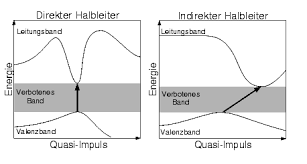
\includegraphics{images/KM2/direkt_indirekt_HL.png}
    \caption{Visualisierung von direkten und indirekten Halbleitern}
    \label{fig:direkte_indirekte_Halbleiter}
\end{figure}
\end{addmargin}

\noindent\textbf{3. Wie hängt die Bandlücke (intrinsischer Halbleiter) von T ab?}\\
\begin{addmargin}[25pt]{0pt}
Für tiefe Temperaturen ($T=0$\,K) ist die Bandlücke proportional zu $T^2$ und für höhere Temperaturen (im Bereich der Raumtemperatur) ist die Bandlücke proportional zu $T$. Dadurch ist die Bandlücke bei Raumtemperatur um 10\% geringer als bei $T=0$\,K. Die dafür verantwortlichen Effekte sind zum einen die thermische Expansion der Probe und dem damit verbunden größerem Abstand benachbarter Atome und zum anderen die Elektron-Phonon-Wechselwirkung.\\
\end{addmargin}

\noindent\textbf{4. Mit welcher Messgröße kann man direkte und indirekte Halbleiter unterscheiden?}\\
\begin{addmargin}[25pt]{0pt}
Man kann den Halbleiter mit elektromagnetischer Strahlung in einem großen Frequenzbereich bestrahlen und die Absorption messen. Ab einer Grenzenergie der Photonen reicht die Energie aus damit die Elektronen die Bandlücke überqueren können und man sieht einen starken Anstieg in der Absorption. Bei direkten Halbleitern steigt Absorption für noch höhere Energien nur noch minimal und kontinuierlich. Andererseits erkennt man in der Absorption von indirekten Halbleitern einen zweiten Absorptionssprung, dieser ist bei der Energie bei der für die Elektronen im indirekten Halbleiter auch ein direkter Übergang zum Leitungsband energetisch möglich wird. (Abbildung \ref{fig:Absorption_HL})\\
\begin{figure}[h]
    \centering
    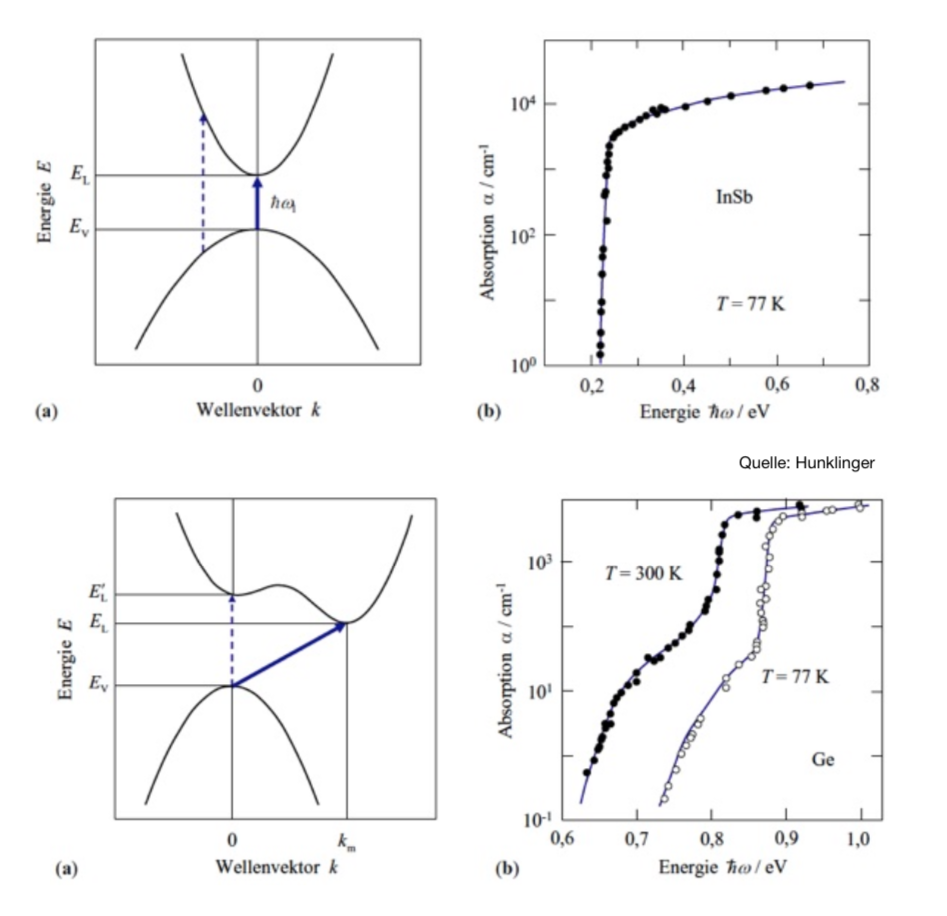
\includegraphics[scale = 0.8]{images/KM2/Absorption_HL.png}
    \caption{Absorptionsmessung für direkte und indirekte Halbleiter}
    \label{fig:Absorption_HL}
\end{figure}
\end{addmargin}

\noindent\textbf{5. Wie verhalten sich die effektiven Massen von intrinsischen Halbleitern?}\\
\begin{addmargin}[25pt]{0pt}
Im Allgemeinen ist die effektive Masse richtungsabhängig. Im Spezialfall der direkten Halbleiter ist der Tensor der effektiven Masse isotrop also richtungsunabhängig. Für den indirekten Halbleiter unterscheidet man zwischen longitudinaler und transversaler effektiver Masse, damit ist dieser Tensor nicht isotrop.  Der Tensor der effektiven Masse berechnet sich mit:
\begin{equation}\label{eq:effektive_Masse}
    m^*_{ij} = \hbar^2 \left(\frac{\partial^2 E}{\partial k_i\partial k_j}\right)^{-1}
\end{equation}
Bei der effektiven Masse ist häufig nur das CBM und VBM relevant da sich die Elektronen und Löcher fast immer in der Nähe dieser Punkte aufhalten.\\

\end{addmargin}

\noindent\textbf{6. Was versteht man unter Eigenleitung von intrinsischen Halbleitern?}\\
\begin{addmargin}[25pt]{0pt}
Die Eigenleitung ist der Teil der Leitfähigkeit, welcher nur durch Anregungen von Elektronen aus den Valenzband in das Leitungsband und Löchern aus dem Leitungsband in das Valenzband entsteht. Zusätzliche Leitfähigkeit wie Effekte durch Verunreinigungen oder Dotierung sind nicht Teil der Eigenleitung. \\
\end{addmargin}

\noindent\textbf{7. Wie hängen die Ladungsträgerkonzentrationen beim intrinsischen Halbleiter von der Temperatur ab?}\\
\begin{addmargin}[25pt]{0pt}
Für einen intrinsischen Halbleiter ist die Dichte der Löcher im Valenzband $p_i$ gleich der Dichte der Elektronen im Leitungsband $n_i$. Aus der Integration der Zustandsdichte über alle erlaubten Energien und unter Berücksichtigung der Fermi-Dirac-Statistik für Fermionen erhält man die Proportionalität:
\begin{equation}\label{eq:Ladungsträgerdichte_intrinsisch_Temperatur}
    n_i = p_i \propto k_BT^{\frac{3}{2}}e^{-\frac{E_g}{2k_bT}}
\end{equation}
Dabei ist $T$ die Temperatur, $k_B$ die Boltzmann-Konstante und $E_g$ die Bandlücke des Halbleiters.\\
\end{addmargin}

\noindent\textbf{8. Was versteht man unter dem Massenwirkungsgesetz?}\\
\begin{addmargin}[25pt]{0pt}
Das Massenwirkungsgesetz besagt, dass das Produkt aus der Elektronendichte im Leitungsband $n$ und der Löcherdichte im Valenzband $p$ eine Konstante ist, welche von den entsprechenden effektiven Massen der Löcher $m_h^*$ und der Elektronen $m_e^*$ abhängt:
\begin{equation}\label{eq:Massenwirkungsgesetz}
    n\cdot p = N_LN_Ve^{-\frac{E_g}{k_BT}}
\end{equation}
Die Konstanten sind ausgeschrieben:
\begin{align}
    N_L = 2\left(\frac{m_e^*k_BT}{2\pi\hbar^2}\right)^{\frac{3}{2}}\\
    N_V = 2\left(\frac{m_h^*k_BT}{2\pi\hbar^2}\right)^{\frac{3}{2}}
\end{align}\\
\end{addmargin}

\noindent\textbf{9. Wo befindet sich das Fermi Niveau beim intrinsischen Halbleiter?}\\
\begin{addmargin}[25pt]{0pt}
Die Fermi-Energie liegt für reine, nicht dotierte Halbleiter ungefähr in der Mitte der Bandlücke. Das ergibt aus Symmetriegründen Sinn, weil für jedes Elektron das vom Valenzband in das Leitungsband angeregt wird auch (ungefähr) ein Loch vom Leitungsband in das Valenzband springt. In der Realität weicht die Fermi-Energie etwas von der Mitte der Bandlücke ab da die Zustandsdichte von den Elektronen im Leitungsband nicht exakt gleich der Zustandsdichte der Löcher im Valenzband ist und somit auch deren Anzahl nach Gleichung \ref{eq:Besetzungszahl_e} und \ref{eq:Besetzungszahl_h} minimal voneinander abweicht:
\begin{align}\label{eq:Besetzungszahl_e}
n_e &= \int\limits_{E_L}^\infty D_L(E)f_{FD}(E,T)\si{d}E\\ \label{eq:Besetzungszahl_h} 
n_h &= \int\limits_{-\infty}^{E_V} D_V(E)\left(1-f_{FD}(E,T)\right)\si{d}E
\end{align}    
Dabei ist $D_V$ die Zustandsdichte der Löcher im Valenzband, $D_L$ die Zustandsdichte der Elektronen im Leitungsband, $E_V$ ist die Energie am VBM, $E_L$ die Energie am CBM und $f_{FD}(E,T) = \frac{1}{e^{\frac{E-E_F}{k_BT}}+1}$ die Fermi-Dirac-Verteilung. Unter Berücksichtigung dieser Zustandsdichten ergibt sich für die Fermi-Energie:
\begin{equation}
    E_{\si{F}} = \frac{E_{\si{V}} + E_{\si{L} }}{2} + \frac{k_BT}{2}\ln{\frac{N_V}{N_L}}
\end{equation}\\
\end{addmargin}

\noindent\textbf{10. Was sind typische Beispiele für dotierte kristalline Halbleiter?}\\
\begin{addmargin}[25pt]{0pt}
Man kann in einen kristallinen Halbleiter Dotieratome einbringen dadurch verändern sich die elektrischen Eigenschaften des Material. Man kann dabei entweder Donatoren oder Akzeptoren einbringen. Donatoren haben mehr Valenzelektronen als zu einer kovalenten Bindung benötigt werden und dadurch hat man mehr freie Elektronen im Kristall. Akzeptoren hingegen haben weniger Elektronen als für eine kovalente Bindung benötigt werden wodurch sie freie Löcher im Kristall erzeugen. Typischerweise nutzt man Phosphor, Arsen, Antimon oder Bismut als Donatoren und Bor, Aluminium, Gallium oder Indium als Akzeptoren. \\
\end{addmargin}

\noindent\textbf{11. Wie groß sind typische Ladungsträgerkonzentrationen beim intrinsischen und dotierten Halbleiter?}\\
\begin{addmargin}[25pt]{0pt}
Die Ladungsträgerkonzentration hängt sehr stark von der Art der Dotieratome und der Konzentration dieser ab. Dadurch kann man eine weite Bandbreite an Ladungsträgerkonzentrationen erreichen. Bei intrinsischen Halbleitern ist die Ladungsträgerkonzentration bei $\approx 10^{19} \frac{1}{\si{m}^3}$ für Germanium, $\approx 10^{16} \frac{1}{\si{m}^3}$ für Silizium und $\approx 10^{12} \frac{1}{\si{m}^3}$ für Gallium-Arsenid. Die besten dotierten Halbleiter von Gallium-Arsenid erreichen sogar $\approx 10^{22} \frac{1}{\si{m}^3}$. Dotierte Silizium -und Germaniumkristalle kommen beide auf $\approx 10^{19} \frac{1}{\si{m}^3}$. Man erkennt also dass sich Germanium sehr schlecht dotieren lässt wohingegen die Ladungsträgerdichte für Gallium-Arsenid um 10 Größenordnungen mit einer Dotierung erhöht werden kann.\\
\end{addmargin}

\noindent\textbf{12. Wie groß sind typische Energieskalen bei dotierten Halbleitern?}\\
\begin{addmargin}[25pt]{0pt}
Eine wichtige Kenngröße für Halbleiter ist die Bindungsenergie der Elektronen/Löcher an die Atome. Das ist die Energie die benötigt wird um ein Elektron vom Valenzband in das Leitungsband zu heben. Wir erwarten bei dotierten Halbleitern eine sehr geringe Bindungsenergie, da bei ihnen ein Loch oder Elektron zusätzlich vorhanden ist und somit dieses nur eine sehr schwache Bindung hat. Diese Vermutung wird von einer Messung bestätigt. Typische Bindungsenergien sind im Bereich von $10$ bis $100 \;\si{ meV}$ \\
\end{addmargin}

\noindent\textbf{13. Wie groß ist der effektive Bohr-Radius eines Dotieratoms?}\\
\begin{addmargin}[25pt]{0pt}
Analog dazu, dass Dotieratome kleine Bindungsenergien haben haben sie auch große effektive Bohr-Radien. Das ist auch intuitiv klar, da schwache Bindung einen großen Abstand zwischen den Bindungspartnern ermöglicht. Dotieratome haben einen effektiven Bohr-Radius der in etwa $50$ bis $100$-mal größer ist als der Bohr-Radius des Wasserstoffatoms.   \\
\end{addmargin}

\noindent\textbf{14. Was versteht man unter \glqq Kompensation\grqq \; bei dotierten Halbleitern?}\\
\begin{addmargin}[25pt]{0pt}
Halbleitermaterialien wie Silizium kann man nicht komplett rein herstellen, also wird es immer Fremdatome in einem Siliziumkristall geben. Dotiert man nun einen solchen Kristall, dann kann es zu Kompensation kommen wenn genauso viele Donatoren wie Akzeptoren in dem Kristall vorhanden sind. Das passiert zum Beispiel, wenn vor der Dotierung nur Donatoren als Fremdatome vorhanden waren und dann mit genauso vielen Akzeptoren dotiert wurde. Das Resultat der Kompensation ist, dass keine freien mehr in dem Kristall vorhanden sind.\\
\end{addmargin}

\noindent\textbf{15. Wie liegen die effektiven Energieniveaus beim dotierten Halbleiter?}\\
\begin{addmargin}[25pt]{0pt}
Bei dotierten Halbleitern entstehen zusätzliche Energieniveaus, dotiert man mit einem Donator so entsteht ein zusätzliches Energieniveau knapp unterhalb des Leitungsbandes und dotiert man mit einem Akzeptor entsteht ein zusätzliches Energieniveau knapp überhalb des Valenzbandes. Diese Niveaus sind in Abbildung \ref{fig:Energieniveaus_Halbleiter} gekennzeichnet.
\begin{figure}[h]
    \centering
    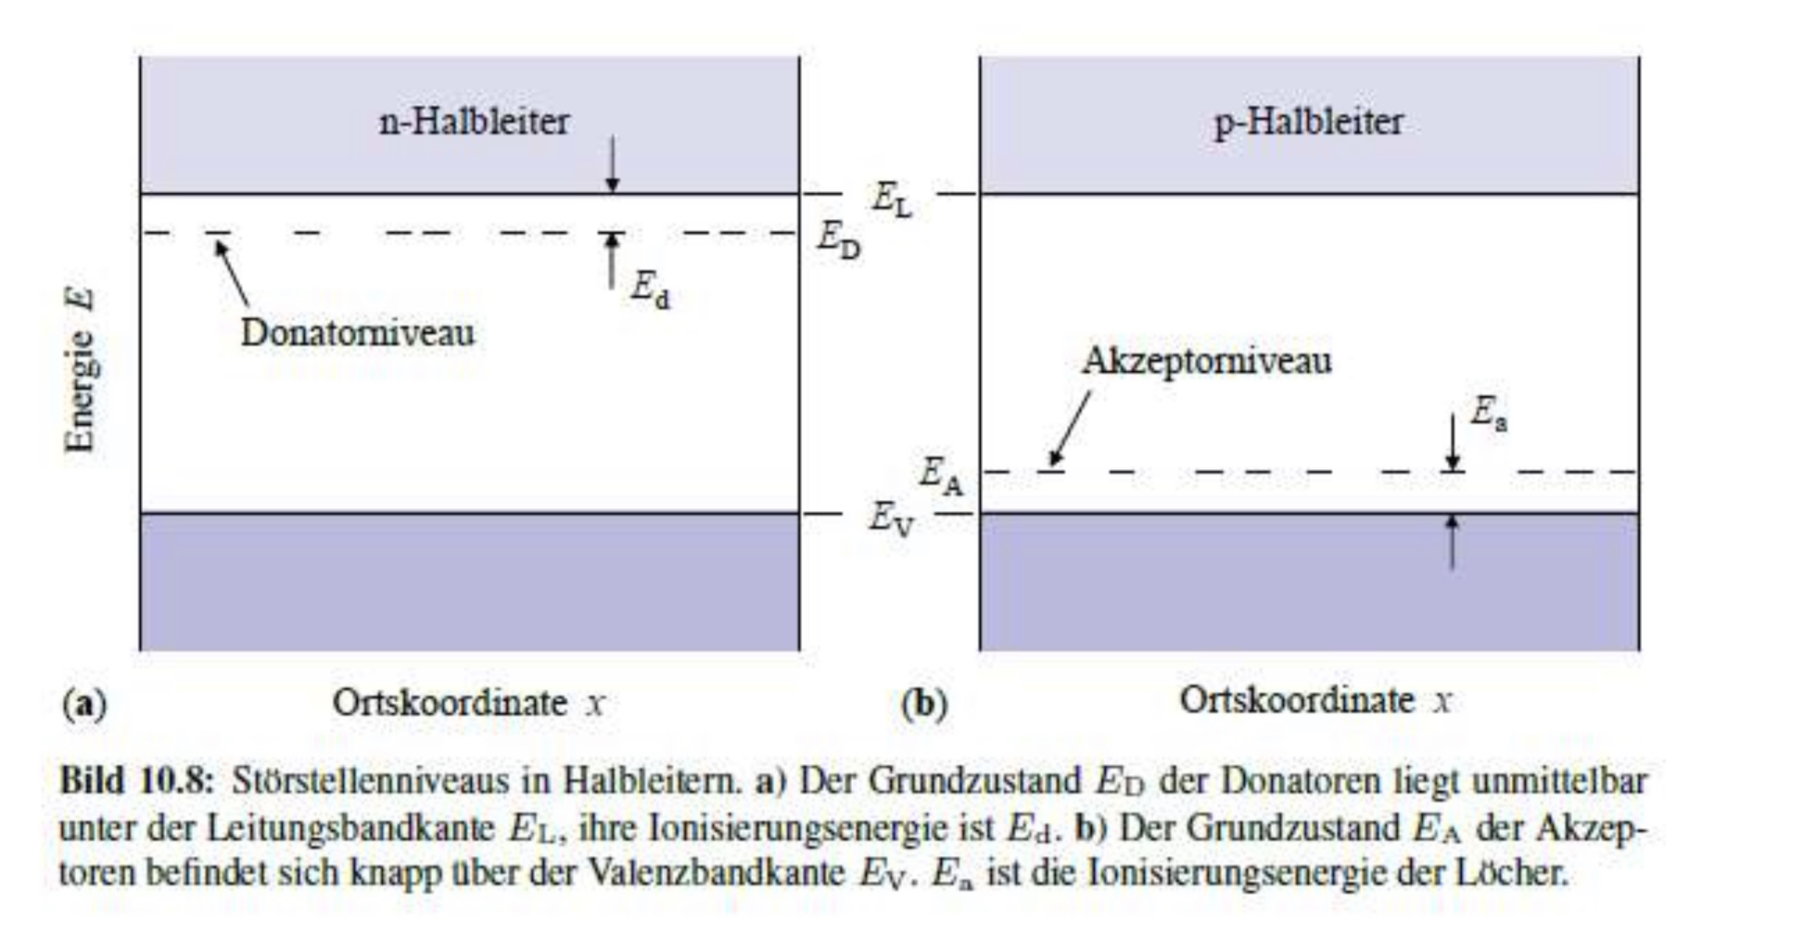
\includegraphics[width = 0.8\textwidth]{images/KM2/Donator_Akzeptorniveaus.jpeg}
    \caption{Darstellung der zusätzlichen Energieniveaus in dotierten Halbleitern}
    \label{fig:Energieniveaus_Halbleiter}
\end{figure}
Eine wichtige Konsequenz dieser zusätzlichen Niveaus ist, dass die Elektronen jetzt nicht mehr die gesamte Bandlücke überwinden müssen um auf ein höheres Niveau zu springen sondern nur noch von $E_V$ zum Akzeptorniveau $E_A$. Analog gilt das ganze für Löcher und das Donatorniveau $E_D$.
\end{addmargin}

\noindent\textbf{16. Was versteht man unter Kompensationsbereich, Störstellenreserve, Erschöpfungszustand und Eigenleitung und wie variiert jeweils die Elektronendichte mit T? }\\
\begin{addmargin}[25pt]{0pt}
In Abbildung \ref{fig:Elektronendichte_T_dotiert} kann man die Abhängigkeit der Elektronendichte von der Temperatur bei einem dotierten Halbleiter sehen, dieser Halbleiter hat einige Akzeptoren als Verunreinigungen in sich aber sehr viele Donatoren durch die Dotierung. In diesem Graphen gibt es 4 Bereiche, bei ganz niedrigen Temperaturen befindet sich der Kompensationsbereich, in diesem gibt es nur sehr wenige freie Ladungsträger und bei steigender Temperatur geben die vorhandenen Donatoren Elektronen ab, diese werden mit gleicher Wahrscheinlichkeit entweder von einem Akzeptor aufgenommen oder stehen als freie Elektronen zur Verfügung. Sobald alle Akzeptoren ein Elektron aufgenommen haben sind immernoch Donatoren verfügbar welche ihr zusätzliches Elektron noch nicht abgegeben haben, bei steigender Temperatur werden auch sie ihr Elektron abgeben und die Anzahl der freien Ladungsträger steigt nun doppelt so stark da abgegebenen Elektronen auch freie Ladungsträger sind. Diesen Bereich nennt man Störstellenreserve. Ab einer gewissen Temperatur haben alle Donatoren ihr Elektron abgegeben, die Elektronendichte bleibt in diesem Erschöpfungszustand für einen gewissen Temperaturbereich konstant. Bei sehr großen Temperaturen kommt es dann zur Eigenleitung, dabei werden dann vom Grundmaterial Ladungsträger direkt in das Leitungsband angelegt.\\
\begin{figure}[h]
    \centering
    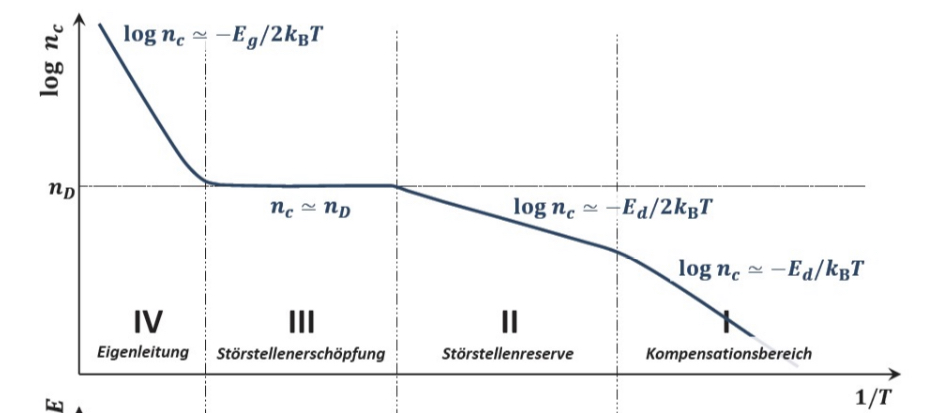
\includegraphics[width = 0.8\textwidth]{images/KM2/Elektronendichte_T_dotierteHL.jpeg}
    \caption{Verhalten der Elektronendichte in Abhängigkeit von der Temperatur bei einem n-Typ halbleiter}
    \label{fig:Elektronendichte_T_dotiert}
\end{figure}
\end{addmargin}

\noindent\textbf{17. Wie verändert sich die Lage des Fermi-Niveaus mit der Temperatur beim dotierten Halbleiter?}\\
\begin{addmargin}[25pt]{0pt}
Der Verlauf der Fermi-Energie in Abhängigkeit von der Temperatur ist in Abbildung \ref{fig:Fermi_Energie_dotiert_Temperatur} dargestellt. Für besonders große Temperaturen, im Bereich der Eigenleitung, befindet sich das Fermi-Niveau in der Mitte des Valenzbands und Leitungsbands, da der Beitrag durch die Elektronen dominiert wird, die vom Valenzband in das Leitungsband angeregt werden. Den Bereich der Störstellenreserve kann man analog beschreiben, allerdings kommen dort alle beteiligten Elektronen aus dem Donatorniveau und somit befindet sich die Fermi-Energie zwischen Donatorniveau und Leitungsband. Erhöht man von der Störstellenreserve die Temperatur werden im Bereich der Störstellenerschöpfung keine Elektronen mehr aus dem Donatorniveau kommen, dafür immer mehr intrinsisch Elektronen, angeregte aus dem Valenzband. Die Fermi-Energie sinkt also Richtung $\frac{E_g}{2}$. Zuletzt muss man noch den Bereich mit sehr kleinen Temperaturen betrachten, den Kompensationsbereich. In diesem Bereich werden, durch die vorhandenen Akzeptoren, nur die Hälfte aller vom Donator freigegebenen Elektronen auch in das Leitungsband angeregt, dadurch ist die Fermi-Energie genau das Donatorniveau.\\ 
\begin{figure}[h]
    \centering
    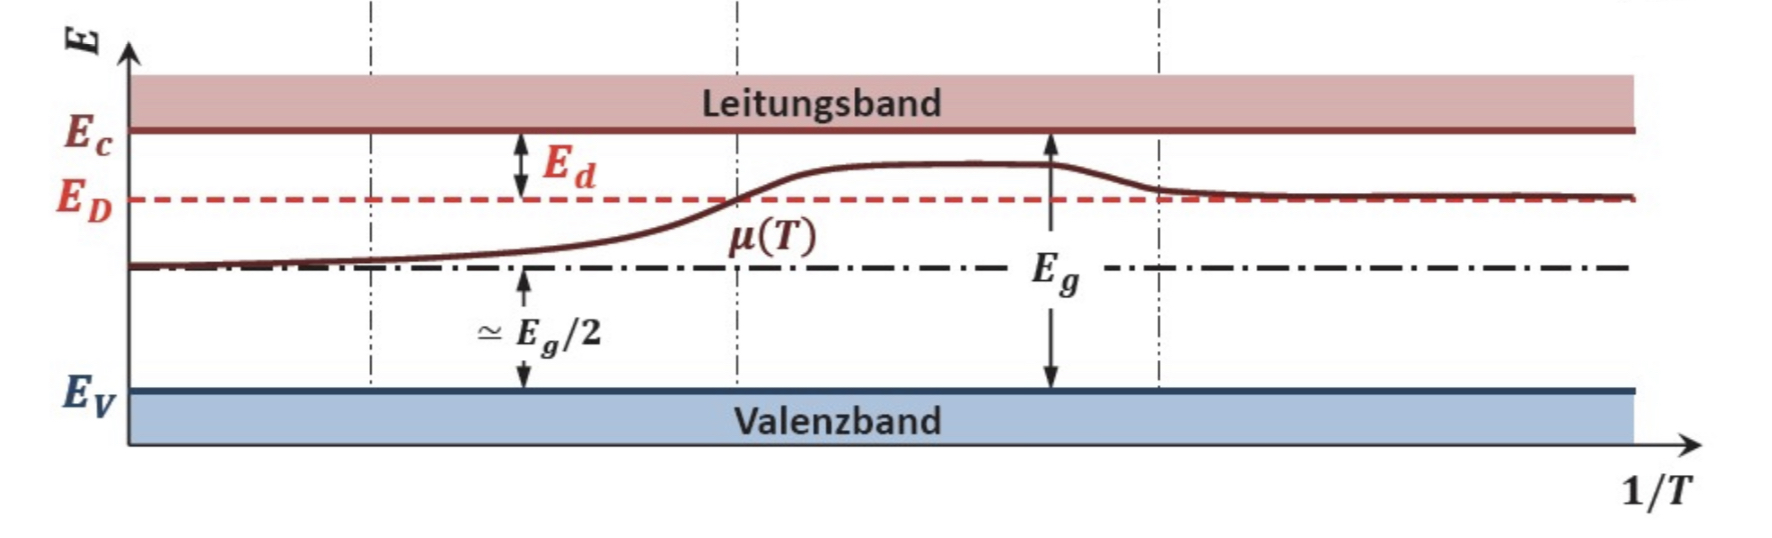
\includegraphics[width = \textwidth]{images/KM2/Fermi_Niveau_Temperatur_dotiert.jpeg}
    \caption{Die Lage des Fermi-Niveaus in den verschiedenen Temperaturbereichen Kompensationsbereich, Störstellenreserve, Störstellenerschöpfung und Eigenleitung für einen n-Typ Halbleiter}
    \label{fig:Fermi_Energie_dotiert_Temperatur}
\end{figure}
\end{addmargin}

\noindent\textbf{18. Wie verändert sich die Beweglichkeit und elektrische Leitfähigkeit mit T?}\\
\begin{addmargin}[25pt]{0pt}
Die Leitfähigkeit $\sigma_i$ hat sowohl einen Anteil von den Elektronen als auch von den Löchern. Sie lautet:
\begin{equation}\label{eq:leitfähigkeit}
    \sigma_i = \sigma_e + \sigma_h = n_i\mu_e e + p_i\mu_h e
\end{equation}
Dabei sind $n_i$ und $p_i$ die schon bekannte Elektronen- und Lochdichte und $\mu_e$ beziehungsweise $\mu_h$ die Beweglichkeiten der Elektronen und Löcher. Die Beweglichkeiten und die Ladungsträgerdichten haben jeweils eine Temperaturabhängigkeit. Die Beweglichkeiten berechnet man mit:
\begin{equation}\label{eq:beweglichkeit_definition}
    \mu_{e|h} = \frac{e\tau_{e|h}}{m^*_{e|h}}
\end{equation}
Dabei ist $\tau_{e|h}$ die temperaturabhängige Stoßzeit zwischen 2 Stößen eines Elektrons bzw. Lochs mit einem Defekt oder einem Phonon. Die Abhängigkeit der Beweglichkeit von der Temperatur ist in Abbildung \ref{fig:Beweglichkeit_Temperatur} dargestellt. Für niedrige Temperaturen dominiert der Anteil der geladenen Störstellen und für hohe Temperaturen der Anteil der Phononen. \\

\begin{figure}[h]
    \centering
    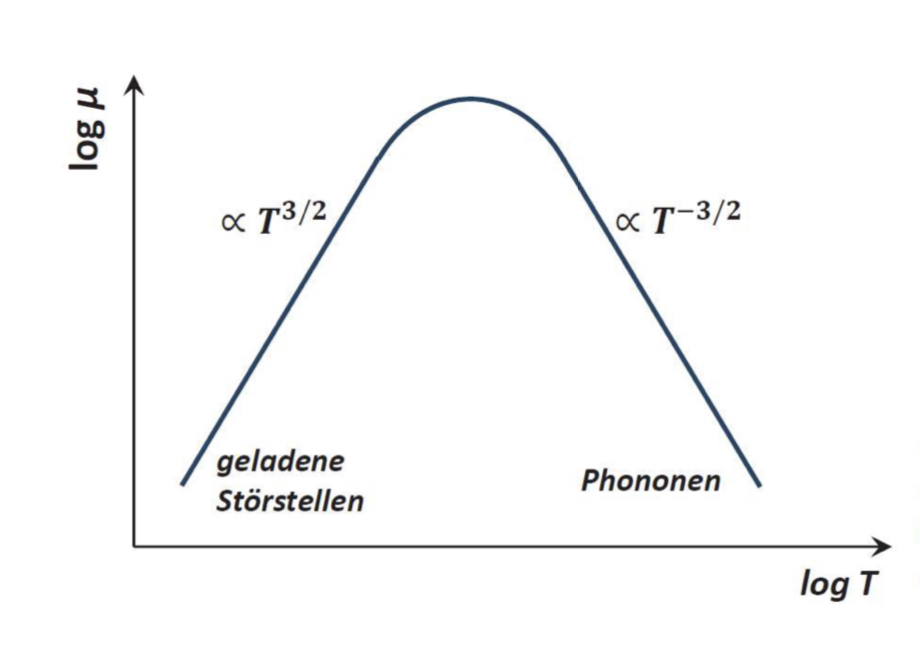
\includegraphics[width = \textwidth]{images/KM2/Beweglichkeit_Temperatur.jpeg}
    \caption{Die Abhängigkeit von der Beweglichkeit von der Temperatur}
    \label{fig:Beweglichkeit_Temperatur}
\end{figure}
\end{addmargin}

\noindent\textbf{19. Welche Rolle spielen Phononen für die Temperaturabhängigkeit der Leitfähigkeit?}\\
\begin{addmargin}[25pt]{0pt}
Phononen haben einen wesentlichen Einfluss auf die Stoßzeit von Elektronen beziehungsweise Löchern bei hohen Temperaturen (siehe Abbildung \ref{fig:Beweglichkeit_Temperatur}). Dadurch haben sie einen direkten Einfluss auf die Beweglichkeit und damit auf die Leitfähigkeit.\\
\end{addmargin}

\noindent\textbf{20. Was versteht man unter inhomogenen Halbleitern?}\\
\begin{addmargin}[25pt]{0pt}
Inhomogene Halbleiter haben keine konstante Dotierung beziehungsweise chemische Zusammensetzung. In dieser Art der Halbleiter können p-dotierte Bereiche direkt neben n-dotierten Bereichen liegen, das nennt man dann einen pn-Übergang. Inhomogene Halbleiter sind in der technischen Anwendung sehr bedeutend.\\
\end{addmargin}

\noindent\textbf{21. Was sind p- und n-Halbleiter?}\\
\begin{addmargin}[25pt]{0pt}
p-Halbleiter sind p-dotierte Halbleiter, also Halbleiter, welche mit Elektronenakzeptoren dotiert wurden. p-Halbleiter sind zum Beipsiel mit Bor, Gallium oder Indium dotiertes Silizium. n-Halbleiter wurden mit Donatoratomen dotiert. n-Halbleiter sind zum Beispiel mit Phosphor, Arsen, oder Antimon dotiertes Silizium.\\
\end{addmargin}

\noindent\textbf{22. Was sind Minoritäts- und Majoritätsladungsträger?}\\
\begin{addmargin}[25pt]{0pt}
Im n-Halbleiter hat man mehr Elektronen als Löcher und im p-Halbleiter ist es exakt anders herum. Die Majoritätsladungsträger sind dann die Art von Ladungsträger die mehr auftritt also Elektronen im n-Halbleiter und Löcher im p-Halbleiter. Die Minoritätsladungsträger sind jeweils die anderen also Löcher im n-Halbleiter und Elektronen im p-Halbleiter.\\
\end{addmargin}

\noindent\textbf{23. Wie verlaufen $E_L$ und $E_V$ beim pn-Übergang?}\\
\begin{addmargin}[25pt]{0pt}
Beim pn-Übergang befindet sich eine abrupte Grenze zwischen einem p-dotierten und einem n-dotierten Bereich (Abbildung \ref{fig:pn-transition}). Dadurch kommt es für die Elektronen und Löcher zu einem Konzentrationsgradienten, sodass die Elektronen nach links in Richtung p-dotierten Bereich diffundieren und die Löcher nach rechts in Richtung n-dotierten Bereich. An der Grenzfläche rekombinieren dann Elektronen mit Löchern, wodurch im p-dotierten Bereich dann Löcher und im n-dotierten Bereich Elektronen zur Ladungsneutralität fehlen. Dadurch ist der n-Bereich positiv und der p-Bereich negativ geladen wodurch sich ein Feld einstellt welches der Teilchendiffusion entgegenwirkt. Dieses entgegenwirkende elektrische Feld bewirkt eine Kraft auf die Löcher des n-Bereichs nach links und auf die Elektronen des p-Bereichs nach rechts. Wie in Abbildung \ref{fig:pn_transition_Raumladung} zu sehen bildet sich dadurch eine Raumladungszone um die Grenzfläche aus. Durch die Verschiebung und Rekombination der Ladungsträger werden auch das Valenz -und das Leitungsband verformt. Der Verlauf der Bänder am pn-Übergang ist in Abbildung \ref{fig:pn_transition_bandverlauf} dargestellt.\\

\begin{figure}[h]
    \centering
    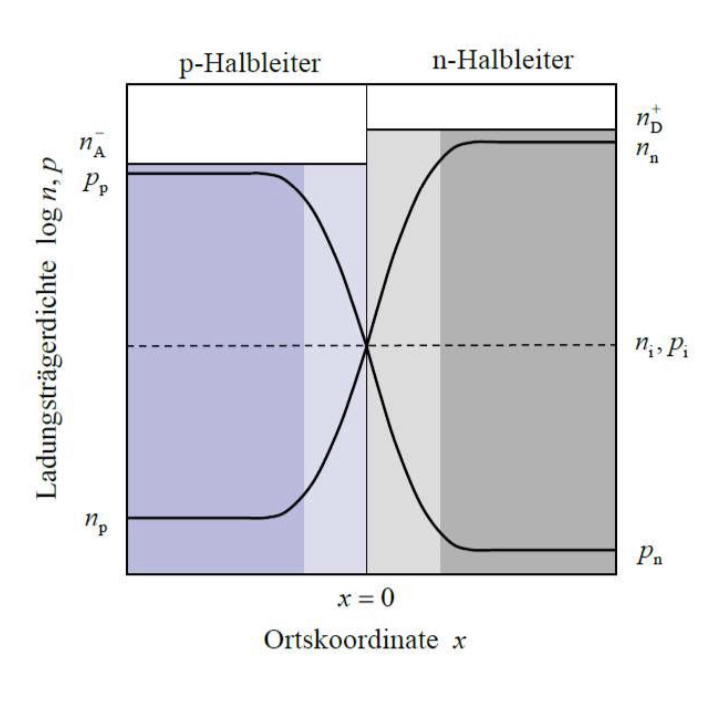
\includegraphics[width = 0.5\textwidth]{images/KM2/pn_transition.jpeg}
    \caption{Visualisierung der Ladungsträgerkonzentrationen beim pn-Üergang}
    \label{fig:pn-transition}
\end{figure}



\begin{figure}[h]
    \centering
    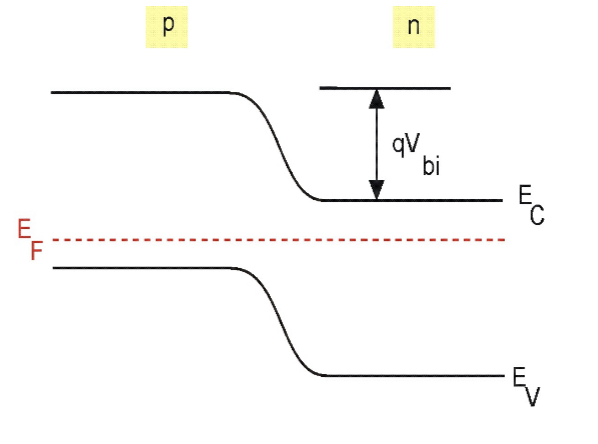
\includegraphics[width = 0.6\textwidth]{images/KM2/pn_transition_bandverlauf.jpeg}
    \caption{Verlauf des Valenzbandes und des Leitungsbandes am pn-Übergang}
    \label{fig:pn_transition_bandverlauf}
\end{figure}
\end{addmargin}
\newpage
\noindent\textbf{24. Was sind die Verarmung und Raumladungszone beim pn-Übergang?}\\
\begin{addmargin}[25pt]{0pt}
Durch die Rekombination von Löchern mit Elektronen sind im p-Bereich weniger Löcher und im n-Bereich weniger Elektronen frei verfügbar. Diese Verringerung an freien Laundgsträgern nennt man Verarmung. Die Raumladungszone ist der Bereich um die Grenzfläche, welcher nach dem Einstellen des Gleichgewichts aus Diffusionsstrom und Gegenfeld eine Nettoladung aufweist. Dieser ist in Abbildung \ref{fig:pn_transition_Raumladung} dargestellt. \\

\begin{figure}[h]
    \centering
    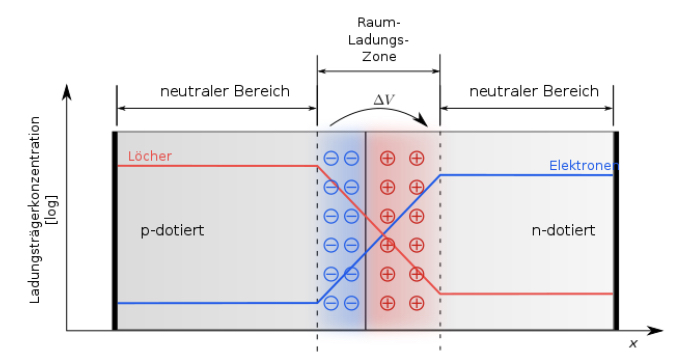
\includegraphics[width = 0.8\textwidth]{images/KM2/pn_transition_Raumladungszone.jpeg}
    \caption{Visualisierung der Raumladungszone beim pn-Übergang}
    \label{fig:pn_transition_Raumladung}
\end{figure}
\end{addmargin}

\noindent\textbf{25. Welche Annahmen werden beim Schottky-Modell des pn-Übergangs gemacht?}\\
\begin{addmargin}[25pt]{0pt}
Das Schottky-Modell nimmt eine scharfe Grenze der Raumladungszone an, also die Ladungsverteilung ist ein Rechteck. Außerdem muss gelten, dass die Gesamtladung der Raumladungszone null ist. Also muss gelten $en_Ad_p = en_Dd_n$, dabei ist $d_p$ die Breite der Raumladungszone von der Grenzfläche zum linken Rand, $d_n$ die Breite von der Grenzfläche zum rechten Rand und $n_A$ beziehungsweise $n_D$ sind die Ladungsträgerdichten im p-Bereich beziehungsweise im n-Bereich. Diesen Ansatz der konstanten, an der Grenze abbrechenden Ladungsverteilungen kann man nun in die Poisson-Gleichung:
\begin{equation}\label{eq:Poissono-Gleichung}
    \frac{\partial^2V(x)}{\partial x^2} = -\frac{\rho(x)}{\epsilon_r\epsilon_0}
\end{equation}
einsetzen und erhält unter Berücksichtigung der Bedingung $V(\infty) - V(-\infty) = V_D$ mit $eV_D = E_{gap}$ einen Ausdruck für die Breite der Raumladungszone:
\begin{equation}\label{eq:Breite_Raumladungszone}
    d_{n,p} = \sqrt{\frac{2\epsilon_r\epsilon_0V_D}{e} \frac{\frac{n_{A,D}}{n_{D,A}}}{n_A + n_D}}
\end{equation}\\
\end{addmargin}

\noindent\textbf{26. Was sind der Diffusionsstrom und der Feldstrom beim pn-Übergang?}\\
\begin{addmargin}[25pt]{0pt}
Der Diffusionsstrom ist der Strom der aufgrund des Konzentrationsgradienten zwischen n- und p-Halbleiter entsteht, er besteht aus den jeweiligen Majoritätsladungsträgern in dem entsprechenden Bereich. Durch die Rekombination an der Grenzfläche entsteht eine positive Nettoladung im n-Bereich und eine negative im p-Bereich, diese Ladungsbereiche rufen ein elektrisches Feld hervor, welches die jeweiligen Minoritätsladungsträger in den einzelnen Bereichen Richtung Grenzfläche verschiebt, diesen Strom aus Minoritätsladungsträgern nennt man Feldstrom. Im thermischen Gelichgewicht sind der Diffusionsstrom und der Feldstrom betragsgleich und entgegengesetzt gerichtet, so entsteht ein stationärer Zustand mit ausgeprägter Raumladungszone.\\
\end{addmargin}

\noindent\textbf{27. Wie verhält sich der pn-Übergang unter einer äußeren Spannung?}\\
\begin{addmargin}[25pt]{0pt}
Wir nehmen an, dass die gesamte Spannung über die Raumladungszone abfällt und der restliche Halbleiter feldfrei ist. Mit dieser Annahme kann man sich überlegen wie sich der pn-Übergang verhält wenn eine Spannung angelegt wird. Dabei muss man 2 Fälle unterscheiden. Im ersten Fall wird der Plus-Pol am p-Halbleiter angelegt und der Minus-Pol am n-Halbleiter, durch diesen Aufbau wird die Dicke der Raumladungszone verringert und es kann ein Strom fließen, das nennt man Durchlassrichtung. Der entgegengesetzte Fall erhöht die Dicke der Raumladungszone, wodurch kein Strom durch durch den pn-Übergang fließen kann. Das nennt man Sperrrichtung. \\
\end{addmargin}

\noindent\textbf{28. Was ist ein Zener-Durchbruch und was eine Zener-Diode?}\\
\begin{addmargin}[25pt]{0pt}
Eine Zener-Diode ist ein pn-Übergang, welcher darauf ausgelegt ist dauerhaft in Sperrrichtung betrieben zu werden. Legt man eine Spannung an dieses Bauteil an, so wird trotzdem kein Strom fließen. Es fließt erst ein Strom wenn die angelegte Spannung einen bestimmten Grenzwert überschreitet. Das geschieht, weil bei diesen hohen Feldern die Elektronen genügend Energie besitzen um durch die Raumladungszone durch zu tunneln. Diesen Durchruch nennt man Zener-Durchbruch.\\
\end{addmargin}

\noindent\textbf{29. Was versteht man unter einem Schottky-Kontakt?}\\
\begin{addmargin}[25pt]{0pt}
Ein Schottky-Kontakt ist ein Bauteil, welches aus einem dotierten Halbleiter und einem Metall besteht. Im Allgemeinen besitzen diese unterschiedlich hohe Fermi-Niveaus. Die Fermi-Niveaus gleichen sich dann an indem Ladungsträger über die Grenzfläche von Metall und Halbleiter diffundieren.\\
\end{addmargin}

\noindent\textbf{30. Was sind Halbleiterheterostrukturen?}\\
\begin{addmargin}[25pt]{0pt}
Halbleiterheterostrukturen sind im einfachsten Fall 2 aneinander gebrachte Halbleiter mit unterschiedlichen Valenzband- und Leitungsbandenergien. Dadurch entstehen Unstetigkeiten am Übergang. Ein Resultat daraus ist, dass im atomaren Bereich sehr hohe elektrische Felder auftreten können. In der Praxis werden diese Bauteile verwendet da sie eine sehr starke Verbesserung der Mobilitäten ermöglichen.\\
\end{addmargin}

\noindent\textbf{31. Was sind dotierungsmodulierte Kompositionsübergitter?}\\
\begin{addmargin}[25pt]{0pt}
Dotierungsmodulierte Kompositionsübergitter sind Verbindungen bei denen abwechselnd Schichten aus einem stark n-dotierten Halbleiter und einem intrinsischen Halbleiter verbaut sind. Der dotierte Halbleiter bildet eine Verarmungszone aus wodurch senkrecht zu den Grenzflächen die Bewegung stark eingeschränkt ist. Allerdings können sich Bloch-Wellen entlang der Grenzfläche sehr gut ausbreiten.  \\
\end{addmargin}

\noindent\textbf{32. Inwiefern beruht eine Solarzelle auf einem pn-Übergang?}\\
\begin{addmargin}[25pt]{0pt}
Eine Solarzelle besteht aus einem pn-Übergang. Ein einfallendes Photon kann, wenn seine Energie größer als die Energie der Bandlücke ist, ein Elektron-Loch Paar in der Raumladunszone erzeugen. Diese freien Ladungsträger werden im E-Feld der Raumladungszone getrennt, so entsteht ein zusätzlicher Strom in Richtung des Feldstroms. Dieser zusätzliche Strom kann über einen Verbraucher abgenommen werden. Allerdings wird ein Teil der erzeugten Ladungsträger wieder rekombinieren bevor er von einem Verbraucher abgegriffen werden kann.\\
\end{addmargin}

\noindent\textbf{33. Wie bestimmt man die maximale Leistung einer Solarzelle?}\\
\begin{addmargin}[25pt]{0pt}
Der Strom in einer Solarzelle hat mehrere Komponenten, eine Komponente durch den pn-Übergang und dessen Diffusions- und Feldstrom und eine Komponente $I_L$ in Richtung des Feldstroms. Der gesamte Strom ist dann:
\begin{equation}\label{eq:Kennlinie_Solarzelle}
    I = I_S\left(e^{\frac{eU}{k_BT}}-1\right) - I_L
\end{equation}
dieser Strom gegen die anliegende Spannung ist in Abbildung \ref{fig:Solarzelle} gezeigt. Die maximale Leistung $P_m$ ist das größte Rechteck was unter diese Kurve passt. Man kann in Abbildung \ref{fig:Solarzelle} auch sehr gut sehen, dass ohne $I_L$ also den Beitrag aus der Photoneneinstrahlung auch keine Leistung umgesetzt werden kann, weil die Kennlinie dann durch den Koordinatenursprung geht. 
\begin{figure}[h]
    \centering
    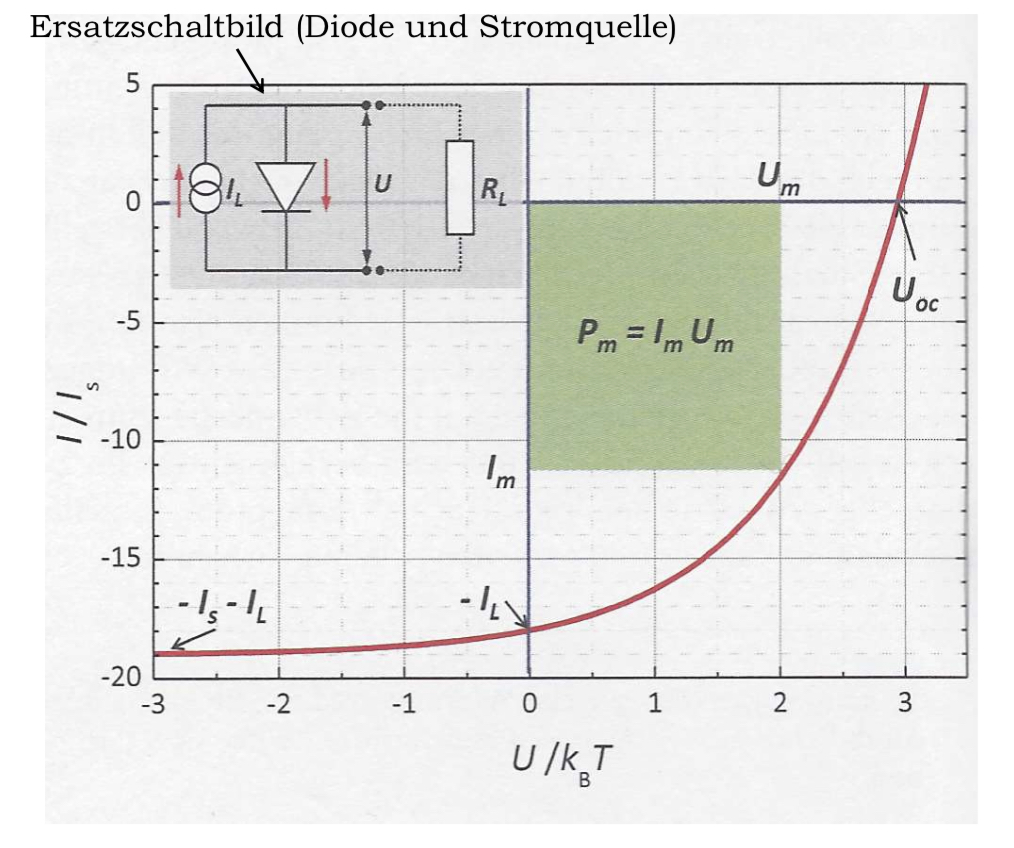
\includegraphics[width = 0.8\textwidth]{images/KM2/Solarzelle.jpeg}
    \caption{Kennlinie einer Solarzelle inklusive Ersatzschaltbild}
    \label{fig:Solarzelle}
\end{figure}
\end{addmargin}

\noindent\textbf{34. Was ist eine Photodiode und wie funktionieren CCD-Sensoren?}\\
\begin{addmargin}[25pt]{0pt}
Eine Photodiode funktioniert prinzipiell wie eine Solarzelle allerdings ist sie deutlich kleiner und wird nicht zur Stromerzeugung sondern zum Nachweis von Licht beispielsweise in Laboren verwendet.\\ 
CCD-Sensoren (charge coupled device) sind eine Matrixanordnung von Photodioden mit denen man nicht nur Licht nachweisen kann sondern dieses auch besser räumlich lokalisieren kann. CCD-Sensoren werden häufig in der Fotografie oder Videotechnik aber auch in Laboren verwendet.
\end{addmargin}

\noindent\textbf{35. Wie funktionieren Leuchtdioden?}\\
\begin{addmargin}[25pt]{0pt}
Leuchtdioden bestehen ebenfalls aus einem pn-Übergang, bei ihnen wird durch ein äußeres elektrisches Feld gezielt eine Rekombination von Elektron mit Loch hervorgerufen, also quasi der umgekehrte Effekt der bei der Solarzelle ausgenutzt wird. Durch diese Rekombination wird ein Photon abgegeben wodurch man aus elektrischem Strom Licht produziert hat. Die Wellenlänge der Photons hängt von der Dotierung, genauer der Bandlücke, der Leuchtdiode ab. \\
\end{addmargin}

\noindent\textbf{36. Was ist ein \glqq transfer resistor\grqq ?}\\
\begin{addmargin}[25pt]{0pt}
Ein \glqq transfer resistor\grqq ist besser bekannt unter dem Namen Transistor. Es gibt pnp- und npn-Transistoren, die sind aus 2 p-dotierten und einem n-dotierten Halbleiter aufgebaut bzw. 2 n-dotierten und einem p-dotierten. Dadurch bilden sich 2 Raumladungszonen aus, diese sind in Abbildung \ref{fig:Transistor}a grau dargestellt. Im Stromkreis wird der pn-Übergang von Emitter zu Basis in der Durchlassrichtung betrieben und der von Kollektor und Basis in der Sperrrichtung. Man kann bei einem Transistor den Stromfluss von Emitter zu Kollektor steuern in dem man einen Basisstrom $I_b$ anlegt. Je nach der Stärke des Basisstroms kann der Stromfluss entweder komplett unterdrückt oder um einen großen Faktor verstärkt werden.\\
\begin{figure}[h]
    \centering
    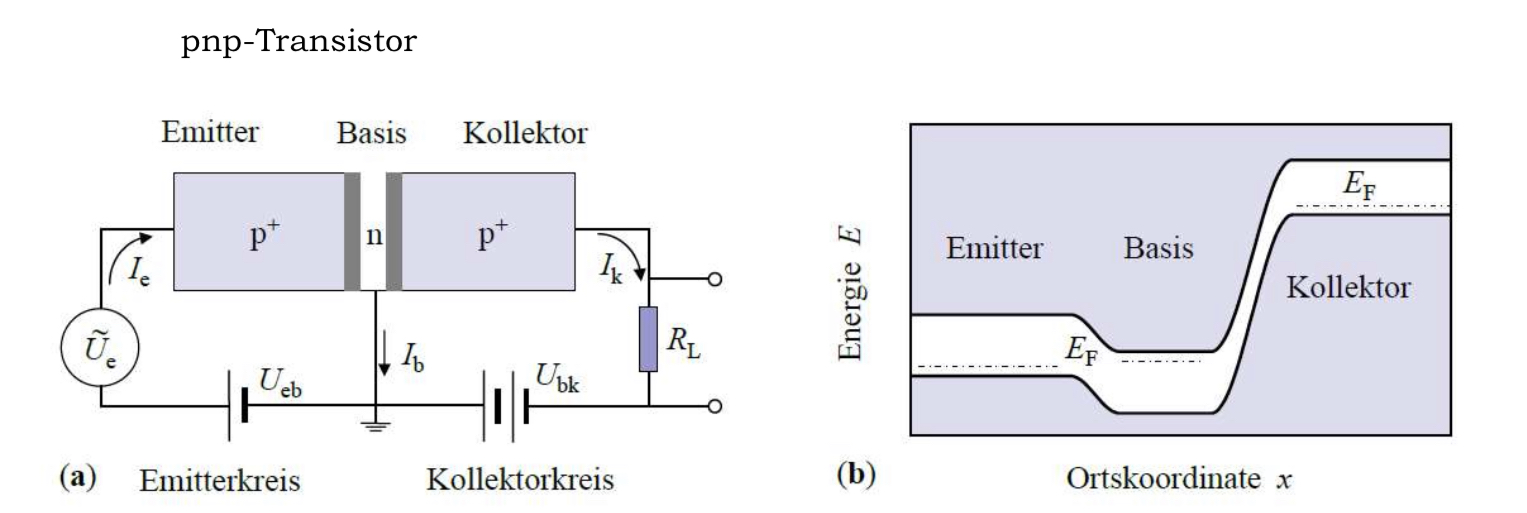
\includegraphics[width = \textwidth]{images/KM2/Transistor.jpeg}
    \caption{(a) schematische Darstellung eines pnp-Transistors in einem Stromkreis (b) Bandschema in einem Transistor}
    \label{fig:Transistor}
\end{figure}
\end{addmargin}

\noindent\textbf{37. Was kann man mit einem pnp-Übergang machen? (Funktionsweise)}\\
\begin{addmargin}[25pt]{0pt}
Mit einem pnp-Übergang kann man einen Stromfluss steuern und verstärken. Der Strom von Emitter zu Kollektor fließt dabei nur wenn auch ein Basisstrom fließt, also eine Spannung zwischen Emitter und Basis anliegt.\\
\end{addmargin}

\noindent\textbf{38. Was ist ein MOSFET und wie funktioniert er?}\\
\begin{addmargin}[25pt]{0pt}
MOSFET steht für Metal-Oxide-Semiconductor Field Effect Transistor. Ein MOSFET hat einen ähnlichen Effekt wie ein pnp- oder npn-Transistor. Wie in Abbildung \ref{fig:MOSFET} dargestellt kann man durch Anlegen einer Spannung $V_g$ an das Gate einen Kanal zwischen Source und Drain erzeugen durch welchen Stromfluss möglich wird. Durch die Stärke der Spannung $V_g$ kann man die Dicke des Kanals und somit die Stärke des Stromflusses bestimmen.\\ 
\begin{figure}[h]
    \centering
    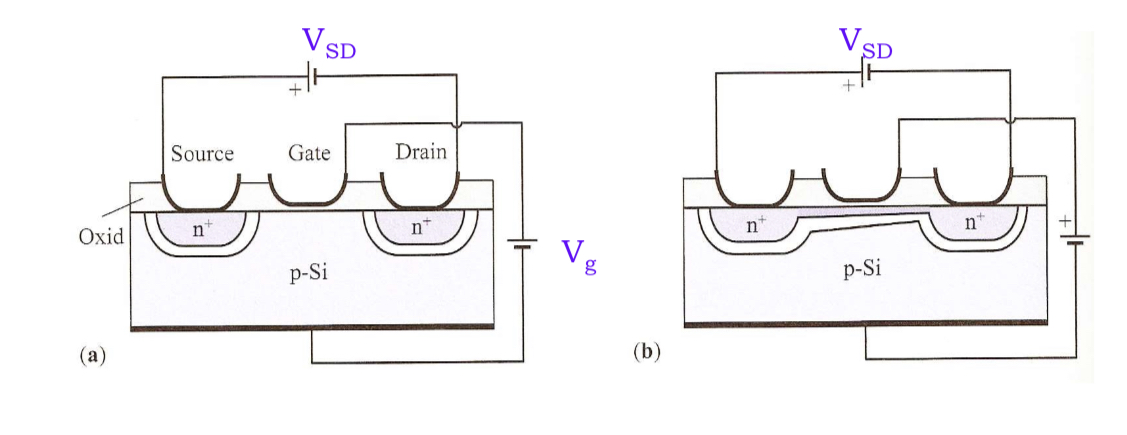
\includegraphics[width = \textwidth]{images/KM2/MOSFET.jpeg}
    \caption{Funktion eines MOSFETs}
    \label{fig:MOSFET}
\end{figure}
\end{addmargin}

\noindent\textbf{39. Wie funktionieren Halbleiterlaser?}\\
\begin{addmargin}[25pt]{0pt}
Ein Halbleiterlaser funktioniert im Prinzip ähnlich wie eine Photodiode nur mit deutlich höheren Intensitäten des Lichts. Diese werden unter Anderem dadurch erreicht, dass reflektierende Schichten die emittierten Photonen zurück in den Laser bringen und dadurch noch deutlich mehr Rekombinationen und schließlich stimulierte Emissionen von Photonen stattfinden können.\\
\end{addmargin}

\subsection{Magnetismus}

\noindent\textbf{1. Welcher Zusammenhang besteht zwischen magnetischem Moment und Drehimpuls?}\\
\begin{addmargin}[25pt]{0pt}
Das magnetische Moment $\vec{\mu}$ ist proportional zum Drehimpuls, dieser ist entweder $\Vec{L}$, $\Vec{S}$ oder $\Vec{J}$. Die Proportionalitätskonstante ist das gyromagnetische Verhältnis $\gamma$ multipliziert mit dem g-Faktor für die Art des Drehimpulses, dieser ist $g_l = 1$, $g_s \approx 2$ und $g_j$ der Landé-Faktor:
\begin{equation}\label{eq:Landé-Faktor}
    g_j = 1 + \frac{j(j+1) + s(s+1) - l(l+1)}{2j(j+1)}
\end{equation}
Das gyromagnetische Verhältnis ist eine Konstante die für das betrachtete Teilchen charakteristisch ist, dieses Verhältnis ist gegeben als:
\begin{equation}\label{eq:gyromagnetisches Verhältnis}
    \gamma = \frac{q}{2m}
\end{equation}
Also ergibt sich für das magnetische Moment für Elektronen $\Vec{\mu}_l$ (Hier beispielhaft für $\Vec{L}$ funktioniert aber analog für $\Vec{S}$ und $\Vec{J}$):
\begin{equation}\label{eq:magnetisches_Moment_Drehimpuls}
    \Vec{\mu}_l = \frac{-e}{2m_e}g_l\Vec{L}
\end{equation}
Durch die Quantisierung des Drehimpulses kann man den Betrag von $\vec{\mu}_l$ finden indem man $|\Vec{L}| = \hbar\sqrt{l(l+1)}$ verwendet:
\begin{equation}\label{eq:Betrag_magnetisches_Moment_Drehimpuls}
    |\Vec{\mu}_l| = \frac{e\hbar}{2m_e}g_l\;\sqrt{l(l+1)} = \mu_B\cdot g_l \cdot\sqrt{l(l+1)}
\end{equation}
Dabei ist $\mu_B = 9,274\cdot 10^{-24} \frac{\si{J}}{\si{T}}$ das \textit{Bohr'sche Magneton}.\\

\end{addmargin}

\noindent\textbf{2. Was ist der Einstein-deHaas-Effekt?}\\
\begin{addmargin}[25pt]{0pt}
Der Einstein-deHaas-Effekt zeigt den Zusammenhang zwischen Magnetimus und Drehimpuls im makroskopischen Bereich. Für dieses Experiment wird ein magnetisierbarer Stab an einen Faden gehangen. Der Stab befindet sich in einer Spule (siehe Abbildung \ref{fig:Einstein_deHaas}), wenn an die Enden der Spule ein Strom angelegt wird baut sich ein, zur Stabachse paralleles, Magnetfeld auf. Durch dieses Magnetfeld richten sich die Spins im Stab aus und dieser ist magnetisiert. Der Stab wird sich dann anfangen um seine Achse zu drehen, das kommt aus der Drehimpulserhaltung. Vor dem Einschalten des B-Feldes war der Gesamtdrehimpuls null und im atomaren die Spins ungeordnet, nach Einschalten des B-Feldes haben sich die Spins ausgerichtet und damit zeigt der Drehimpuls jedes Atoms in die selbe Richtung, aus der Drehimpulserhaltung folgt nun dass sich der Stab makroskopisch anfangen muss zu drehen.\\
\begin{figure}[h]
    \centering
    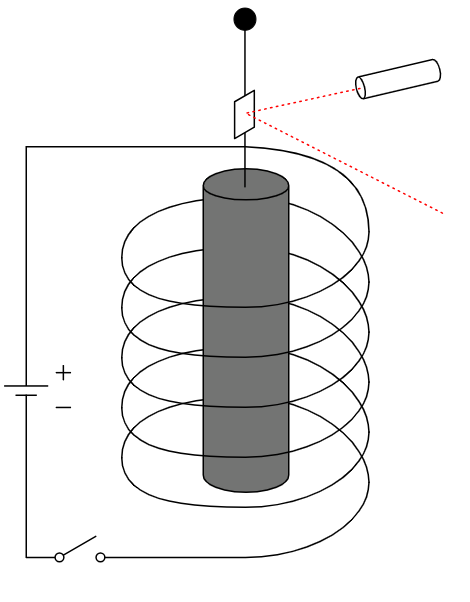
\includegraphics[width = 0.5\textwidth]{images/KM2/Einstein_deHaas.png}
    \caption{Der Versuchsaufbau des Einstein-deHaas-Effekts}
    \label{fig:Einstein_deHaas}
\end{figure}
\end{addmargin}
\vspace{5cm}
\noindent\textbf{3. Was ist die Larmor Präzession und die Larmor-Frequenz?}\\
\begin{addmargin}[25pt]{0pt}
Befindet sich ein Teilchen mit magnetischem Moment $\vec{\mu}$ in einem äußeren Magnetfeld $\Vec{B}$ so erfährt sein Drehimpuls eine Änderung aufgrund des Drehmoments $\Vec{M} = \Vec{\mu} \times \Vec{B}$. Eingesetzt in die Bewegungsgleichungen findet man: 
\begin{equation}\label{eq:Bewegungsgleichung_Larmor}
    \frac{\si{d}\vec{\mu}}{\si{d}t} = \gamma \Vec{\mu} \times \Vec{B}
\end{equation}
Daraus sieht man, dass die Änderung des magnetischen Moments senkrecht auf $\Vec{\mu}$ und $\Vec{B}$ steht, also das magnetische Moment präzediert um das äußere Magnetfeld. Die Frequenz dieser Larmor-Präzession nennt man Larmor-Frequenz:
\begin{equation}\label{eq:Larmor_Frequenz}
    \omega_L = \frac{eB}{2m_e}
\end{equation}
\end{addmargin}

\noindent\textbf{4. Wie hängen Magnetisierung und magnetisches Moment zusammen?}\\
\begin{addmargin}[25pt]{0pt}
Jedes Atom trägt in einem Festkörper ein magnetisches Moment. Dadurch hat der Festkörper im gesamten auch ein magnetisches Verhalten, dieses wird durch die Magnetisierung dargestellt. Die Magentisierung $\Vec{M}$ ist dabei ein Maß für die Menge an atomarem magnetischem Moment pro Volumen. Sie ist ein glattes Vektorfeld und wird berechnet mit:
\begin{equation}\label{eq:Definition_Magnetisierung}
    \Vec{M} = \frac{\partial \Vec{\mu}}{\partial V}
\end{equation}

\end{addmargin}

\noindent\textbf{5. Was sind Entmagnetisierungsfelder und Entmagnetisierungsfaktoren?}\\
\begin{addmargin}[25pt]{0pt}
Legt man ein äußeres Magnetfeld $\vec{B}_a$, $\Vec{H}_a$ an ein Material an, so wird aufgrund der Interaktion des äußeren Magnetfeldes mit den Atomen des Körpers das Magnetfeld im Körperinneren $\vec{B}_i$, $\Vec{H}_i$ ungleich dem von außen angelegten sein. Mit der Magnetisierung $\Vec{M}$ ergibt sich dann:
\begin{align}
    \Vec{H}_i &= \Vec{H}_a - N\cdot\Vec{M}\\
    \Vec{B}_i &= \Vec{B}_a + \mu_0 (1-N)\Vec{M}
\end{align}
In diesen Gleichungen nennt man $\Vec{H}_d = N\cdot\Vec{M}$ das Entmagnetisierungsfeld und $N$ den Entmagnetisierungsfaktor, dieser hängt dabei von der Geometrie des Körpers ab, für eine Kugel gilt zum Beispiel $N = \frac{1}{3}$.\\ 
\end{addmargin}

\noindent\textbf{6. Was besagt das Bohr-van-Leeuwen-Theorem?}\\
\begin{addmargin}[25pt]{0pt}
Das Bohr-van-Leeuwen-Theorem besagt, dass unter der Annahme von klassischen, nicht-wechselwirkenden Elektronen im Magnetfeld die Magnetisierung des Festkörpers exakt verschwindet. Das bedeutet, dass Magnetismus nicht mit der klassischen Physik erklärt werden kann sondern eine quantenmechanische Beschreibung der Systeme notwendig ist. In der Herleitung dieses Sachverhaltes stellt man die kanonische Zustandssumme basierend auf dem klassischen Hamilton-Operator auf. Man stellt fest, dass diese nicht mehr vom magnetischen Feld abhängt und somit die Magnetisierung, welche die Ableitung der freien Energie nach dem B-Feld ist, null sein muss. Die freie Energie ist proportional zum Logarithmus der Zustandssumme.  \\
\end{addmargin}

\noindent\textbf{7. Was sind \glqq skipping orbits\grqq ?}\\
\begin{addmargin}[25pt]{0pt}
Liegt ein Magnetfeld an einer Probe an, so bewegen sich nach klassischer Erwartung die Elektronen in der Probe auf Kreisbahnen. Dabei tritt ein Problem auf: Elektronen, welche sich nah am Rand der Probe befinden, müssten auf ihrer Kreisbahn den Körper verlassen und das ist nicht möglich. Diese Elektronen werden beim Auftreffen auf den Rand der Probe reflektiert und bewegen sich anschließend weiter auf einer Kreisbahn, da sie keine komplette Kreisbewegung vollführen sondern diese immer unterbrochen und neu angesetzt wird nennt man ihre Bewegung \glqq skipping orbits\grqq  \\
\end{addmargin}

\noindent\textbf{8. Wodurch entstehen die diamagnetische und paramagnetische Suszeptibilität isolierter magnetischer Momente?}\\
\begin{addmargin}[25pt]{0pt}
Paramagnetismus tritt nur in Materialien auf, welche ungepaarte Atome besitzen und ein magnetisches Moment besitzen. Die Elementarmagnete der Probe besitzen keine Ausrichtung ohne äußeres Feld. Legt man ein magnetisches äußeres Feld an, so richten sich  die Elementarmagnete bevorzugt mit der Richtung der Feldlinien aus. Für Paramagneten ist die Suszeptibilität $\chi >0$. Diamagnetismus entsteht in allen Materialien, allerdings ist der Effekt des Diamagnetismus so schwach, dass er nur relevant wird in Materialien die weder paramagnetisch noch ferromagnetisch sind. Für die diamagnetische Suszeptibilität gilt $\chi <0$. Diamagnete haben ebenso nur eine Ausrichtung der Elementarmagnete durch ein äußeres magnetisches Feld, bei ihnen richten sich die Elementarmagnete jedoch antiparallel zum äußeren B-Feld aus.\\
\end{addmargin}

\noindent\textbf{9. Wie hängen Diamagnetismus und Kernladungszahl zusammen?}\\
\begin{addmargin}[25pt]{0pt}
Antwort\\
\end{addmargin}

\noindent\textbf{10. Was beschreibt die Langevin-Gleichung?}\\
\begin{addmargin}[25pt]{0pt}
Antwort\\
\end{addmargin}

\noindent\textbf{11. Was beschreibt die Brillouin Funktion?}\\
\begin{addmargin}[25pt]{0pt}
Antwort\\
\end{addmargin}

\noindent\textbf{12. Was versteht man unter Curie-Verhalten?}\\
\begin{addmargin}[25pt]{0pt}
Das Curie-Gesetz besagt, dass die paramagnetische Suszeptibilität invers proportional zur Temperatur ist im Fall von großen Temperaturen oder kleinen Magnetfeldern. Das Curie-Gesetz beschreibt einen Festkörper bei dem der gesamte magnetische Effekt auf den Elektronen mit Spin $\frac{1}{2}$ beruht. Das Curie-Gesetz lautet als Formel:
\begin{equation}\label{eq:Curie-Gesetz}
    \chi = \frac{C}{T}
\end{equation}
Dabei ist $C = \mu_0\frac{N}{V}\frac{(g_j\mu_B)^2}{3}\frac{j(j+1)}{k_B}$ die Curie-Konstante. $\frac{N}{V}$ ist dabei die Anzahl an Teilchen pro Volumen im Festkörper und $\mu_0 = 4\pi\cdot 10^{-7} \frac{\si{kg}\cdot \si{m}}{\si{A}^2\cdot \si{s}^2}$ ist die magnetische Feldkonstante. $k_B = 1,38\cdot 10^{-23} \frac{\si{J}}{\si{K}}$ ist die Boltzmann-Konstante.\\
\end{addmargin}

\noindent\textbf{13. Was ist van Vleck Paramagnetismus?}\\
\begin{addmargin}[25pt]{0pt}
Antwort\\
\end{addmargin}

\noindent\textbf{14. Was besagen die Hund'schen Regeln für die magnetischen Momente von Atomen?}\\
\begin{addmargin}[25pt]{0pt}
Antwort\\
\end{addmargin}

\noindent\textbf{15. Was versteht man unter Kristallfeldern?}\\
\begin{addmargin}[25pt]{0pt}
Antwort\\
\end{addmargin}

\noindent\textbf{16. Welchen Einfluss haben die Kristallfelder auf die magnetischen Eigenschaften?}\\
\begin{addmargin}[25pt]{0pt}
Antwort\\
\end{addmargin}

\noindent\textbf{17. Was sind high-spin und low-spin Zustände bei Eisen?}\\
\begin{addmargin}[25pt]{0pt}
Antwort\\
\end{addmargin}

\noindent\textbf{18. Was versteht man unter \glqq orbitalem Quenchen\grqq ?}\\
\begin{addmargin}[25pt]{0pt}
Antwort\\
\end{addmargin}

\noindent\textbf{19. Was ist der Jahn-Teller-Effekt?}\\
\begin{addmargin}[25pt]{0pt}
Antwort\\
\end{addmargin}

\noindent\textbf{20. Welche Rolle spielen dipolare Wechselwirkungen für die magnetische Ordnung?}\\
\begin{addmargin}[25pt]{0pt}
Antwort\\
\end{addmargin}

\noindent\textbf{21. Was versteht man unter Austauschwechselwirkung?}\\
\begin{addmargin}[25pt]{0pt}
Antwort\\
\end{addmargin}

\noindent\textbf{22. Was beschreibt das Heisenberg-Modell?}\\
\begin{addmargin}[25pt]{0pt}
Antwort\\
\end{addmargin}

\noindent\textbf{23. Was sind direkter und indirekter Austausch?}\\
\begin{addmargin}[25pt]{0pt}
Antwort\\
\end{addmargin}

\noindent\textbf{24. Was sind Superaustausch, Doppelaustausch und anisotroper Austausch?}\\
\begin{addmargin}[25pt]{0pt}
Antwort\\
\end{addmargin}

\noindent\textbf{25. Welche Annahmen macht das Weiss-Modell des Ferromagnetismus?}\\
\begin{addmargin}[25pt]{0pt}
Antwort\\
\end{addmargin}

\noindent\textbf{26. Welchen Einfluss hat ein Magnetfeld auf Ferromagnetismus?}\\
\begin{addmargin}[25pt]{0pt}
Antwort\\
\end{addmargin}

\noindent\textbf{27. Was ist ein Molekularfeld im Weiss-Modell?}\\
\begin{addmargin}[25pt]{0pt}
Antwort\\
\end{addmargin}

\noindent\textbf{28. Was beschreibt die \glqq staggered magnetization\grqq ?}\\
\begin{addmargin}[25pt]{0pt}
Antwort\\
\end{addmargin}

\noindent\textbf{29. Was sind ein \glqq Spin-Flop\grqq\; und ein \glqq Spin-Flip\grqq \; Übergang?}\\
\begin{addmargin}[25pt]{0pt}
Antwort\\
\end{addmargin}

\noindent\textbf{30. Welche Rolle spielen Symmetriebrechungen bei magnetischer Ordnung?}\\
\begin{addmargin}[25pt]{0pt}
Antwort\\
\end{addmargin}

\noindent\textbf{31. Was versteht man unter einem Ordnungsparameter?}\\
\begin{addmargin}[25pt]{0pt}
Antwort\\
\end{addmargin}

\noindent\textbf{32. Was versteht man unter Landau-Theorie und was unter Molekularfeldtheorie?}\\
\begin{addmargin}[25pt]{0pt}
Antwort\\
\end{addmargin}

\noindent\textbf{33. Was versteht man unter dem Ising-Modell?}\\
\begin{addmargin}[25pt]{0pt}
Antwort\\
\end{addmargin}

\noindent\textbf{34. Was sind Magnonen und wie sieht deren Dispersion aus?}\\
\begin{addmargin}[25pt]{0pt}
Antwort\\
\end{addmargin}

\noindent\textbf{35. Was beschreibt das Bloch $T^{\frac{3}{2}}$-Gesetz?}\\
\begin{addmargin}[25pt]{0pt}
Antwort\\
\end{addmargin}

\noindent\textbf{36. Was sind magnetische Domänen und wodurch entstehen sie?}\\
\begin{addmargin}[25pt]{0pt}
Antwort\\
\end{addmargin}

\noindent\textbf{37. Was versteht man unter magnetischer Anisotropie?}\\
\begin{addmargin}[25pt]{0pt}
Antwort\\
\end{addmargin}


\subsection{Supraleitung}
\noindent\textbf{1. Wie weißt man das Verschwinden des elektrischen Widerstandes im Supraleiter nach?}\\
\begin{addmargin}[25pt]{0pt}
Dafür verwendet man einen Ring aus supraleitendem Material und erzeugt in diesem ein Magnetfeld, die Anordnung befindet sich bei einer Temperatur oberhalb der kritischen Temperatur. Danach kühlt man das System auf $T<T_C$ und schaltet das Magnetfeld ab. Basierend auf den Erkenntnissen der Elektrodynamik würde man in diesem Ring einen exponentiell abklingenden induzierten Strom nach der Formel $I(t) = I_0 \exp\left(-\frac{Rt}{L}\right)$ erwarten. Im supraleitenden Material hingegen misst man einen nicht abfallenden induzierten Strom was zeigt, dass im Supraleiter tatsächlich exakt $R=0$ gilt. \\
\end{addmargin}

\noindent\textbf{2. Was ist der Meißner-Ochsenfeld-Effekt?}\\
\begin{addmargin}[25pt]{0pt}
Antwort\\
\end{addmargin}

\noindent\textbf{3. Was unterscheidet ideale Diamagnete von Supraleitern?}\\
\begin{addmargin}[25pt]{0pt}
Antwort\\
\end{addmargin}

\noindent\textbf{4. Wie sieht das Phasendiagramm von Supraleitern aus?}\\
\begin{addmargin}[25pt]{0pt}
Antwort\\
\end{addmargin}

\noindent\textbf{5. Was beschreiben die London-Gleichungen?}\\
\begin{addmargin}[25pt]{0pt}
Antwort\\
\end{addmargin}

\noindent\textbf{6. Was versteht man unter der Londonschen Eindringtiefe?}\\
\begin{addmargin}[25pt]{0pt}
Antwort\\
\end{addmargin}

\noindent\textbf{7. Wie hängt die Enthalpie des Supraleiters vom kritischen Magnetfeld ab?}\\
\begin{addmargin}[25pt]{0pt}
Antwort\\
\end{addmargin}

\noindent\textbf{8. Wie weißt man Supraleiter als thermodynamische Ordnung nach?}\\
\begin{addmargin}[25pt]{0pt}
Antwort\\
\end{addmargin}

\noindent\textbf{9. Was versteht man unter dem Isotopeneffekt?}\\
\begin{addmargin}[25pt]{0pt}
Antwort\\
\end{addmargin}

\noindent\textbf{10. Was sind Cooper-Paare?}\\
\begin{addmargin}[25pt]{0pt}
Antwort\\
\end{addmargin}

\noindent\textbf{11. Welcher Zusammenhang besteht zwischen Cooper-Paaren und der Gesamtwellenfunktion?}\\
\begin{addmargin}[25pt]{0pt}
Antwort\\
\end{addmargin}

\noindent\textbf{12. Welche Annahme macht die BCS-Theorie über die Elektron-Elektron Wechselwirkung?}\\
\begin{addmargin}[25pt]{0pt}
Antwort\\
\end{addmargin}

\noindent\textbf{13. Was zeichnet den BCS Grundzustand aus?}\\
\begin{addmargin}[25pt]{0pt}
Antwort\\
\end{addmargin}

\noindent\textbf{14. Was versteht man unter der supraleitenden Kondensationsenergie?}\\
\begin{addmargin}[25pt]{0pt}
Antwort\\
\end{addmargin}

\noindent\textbf{15. Wie hängt die Energiedichte mit der Zustandsdichte zusammen?}\\
\begin{addmargin}[25pt]{0pt}
Antwort\\
\end{addmargin}

\noindent\textbf{16. Wie verläuft die Dispersion ungepaarter Elektronen im Supraleiter?}\\
\begin{addmargin}[25pt]{0pt}
Antwort\\
\end{addmargin}

\noindent\textbf{17. Wie hängen Energiedichte und supraleitende Übergangstemperatur zusammen?}\\
\begin{addmargin}[25pt]{0pt}
Antwort\\
\end{addmargin}

\noindent\textbf{18. Wie kann man die Energiedichte experimentell nachweisen?}\\
\begin{addmargin}[25pt]{0pt}
Antwort\\
\end{addmargin}

\noindent\textbf{19. Was versteht man unter Tunnelkontakt-Spektroskopie?}\\
\begin{addmargin}[25pt]{0pt}
Antwort\\
\end{addmargin}

\noindent\textbf{20. Was bestimmt die kritische Stromstärke des Supraleiters?}\\
\begin{addmargin}[25pt]{0pt}
Antwort\\
\end{addmargin}

\noindent\textbf{21. Was versteht man unter Flussquantisierung des Supraleiters?}\\
\begin{addmargin}[25pt]{0pt}
Antwort\\
\end{addmargin}

\noindent\textbf{22. Was versteht man unter dem Josephson-Gleichstrom Effekt?}\\
\begin{addmargin}[25pt]{0pt}
Antwort\\
\end{addmargin}

\noindent\textbf{23. Was versteht man unter Josephson Wechselstrom}\\
\begin{addmargin}[25pt]{0pt}
Antwort\\
\end{addmargin}

\noindent\textbf{24. Wie verhält sich ein Josephson-Kontakt im Magnetfeld?}\\
\begin{addmargin}[25pt]{0pt}
Antwort\\
\end{addmargin}

\noindent\textbf{25. Was besagen die Ginzburg-Landau Gleichungen?}\\
\begin{addmargin}[25pt]{0pt}
Antwort\\
\end{addmargin}

\noindent\textbf{26. Was versteht man unter Ginzburg-Landau Eindringtiefe?}\\
\begin{addmargin}[25pt]{0pt}
Antwort\\
\end{addmargin}

\noindent\textbf{27. Was ist die Kohärenzlänge des Supraleiters?}\\
\begin{addmargin}[25pt]{0pt}
Antwort\\
\end{addmargin}

\noindent\textbf{28. Wie ist der Ginzburg-Landau Parameter definiert?}\\
\begin{addmargin}[25pt]{0pt}
Antwort\\
\end{addmargin}

\noindent\textbf{29. Was sind Typ-2-Supraleiter?}\\
\begin{addmargin}[25pt]{0pt}
Antwort\\
\end{addmargin}

\noindent\textbf{30. Wie sieht das Phasendiagramm des Typ-2-Supraleiters aus?}\\
\begin{addmargin}[25pt]{0pt}
Antwort\\
\end{addmargin}

\noindent\textbf{31. Was versteht man unter einem Abrikossow-Gitter}\\
\begin{addmargin}[25pt]{0pt}
Antwort\\
\end{addmargin}

\noindent\textbf{32. Was ist flux flow?}\\
\begin{addmargin}[25pt]{0pt}
Antwort\\
\end{addmargin}

\subsection{Oberflächen}
\noindent\textbf{1. Nenne Sie wichtige Beispiele für typische Flächenfüllungen von Oberflächen!}\\
\begin{addmargin}[25pt]{0pt}
Antwort\\
\end{addmargin}

\noindent\textbf{2. Was versteht man unter einer Oberflächenrekonstruktion?}\\
\begin{addmargin}[25pt]{0pt}
Antwort\\
\end{addmargin}

\noindent\textbf{3. Was versteht man unter einer (2x1)-Rekonstruktion?}\\
\begin{addmargin}[25pt]{0pt}
Antwort\\
\end{addmargin}

\noindent\textbf{4. Wodurch kommen Oberflächen-Rekonstruktionen zustande?}\\
\begin{addmargin}[25pt]{0pt}
Antwort\\
\end{addmargin}

\noindent\textbf{5. Was sind symmetrische und asymmetrische Dimer?}\\
\begin{addmargin}[25pt]{0pt}
Antwort\\
\end{addmargin}

\noindent\textbf{6. Was sind inkommensurable Rekonstruktionen?}\\
\begin{addmargin}[25pt]{0pt}
Antwort\\
\end{addmargin}

\noindent\textbf{7. Wie bezeichnet man primitive, zentrierte und gedrehte Einheitszellen?}\\
\begin{addmargin}[25pt]{0pt}
Antwort\\
\end{addmargin}

\noindent\textbf{8. Was sind vizinale Oberflächen?}\\
\begin{addmargin}[25pt]{0pt}
Antwort\\
\end{addmargin}

\noindent\textbf{9. Welche typischen Defekte von Oberflächen gibt es?}\\
\begin{addmargin}[25pt]{0pt}
Antwort\\
\end{addmargin}

\noindent\textbf{10. Was versteht man unter dem Vakuumleitwert?}\\
\begin{addmargin}[25pt]{0pt}
Antwort\\
\end{addmargin}

\noindent\textbf{11. Wie berechnen sich Vakuumleitwerte für Parallel- und Reihenschaktungen? }\\
\begin{addmargin}[25pt]{0pt}
Antwort\\
\end{addmargin}

\noindent\textbf{12. Wie lautet die Pumpgleichung?}\\
\begin{addmargin}[25pt]{0pt}
Antwort\\
\end{addmargin}

\noindent\textbf{13. Was sind typische UHV-taugliche Materialien?}\\
\begin{addmargin}[25pt]{0pt}
Antwort\\
\end{addmargin}

\noindent\textbf{14. Wie funktionieren Drehschieber-, Turbomolekular- und Ionengitterpumpen?}\\
\begin{addmargin}[25pt]{0pt}
Antwort\\
\end{addmargin}

\noindent\textbf{15. Wie funktionieren Pirani- und Baxard-Alpert-Röhren}\\
\begin{addmargin}[25pt]{0pt}
Antwort\\
\end{addmargin}

\noindent\textbf{16. Was versteht man unter LEED?}\\
\begin{addmargin}[25pt]{0pt}
Antwort\\
\end{addmargin}

\noindent\textbf{17. Welche Informationen liefert LEED?}\\
\begin{addmargin}[25pt]{0pt}
Antwort\\
\end{addmargin}

\noindent\textbf{18. Was versteht man unter RHEED?}\\
\begin{addmargin}[25pt]{0pt}
Antwort\\
\end{addmargin}

\noindent\textbf{19. Was versteht man unter GIXRD?}\\
\begin{addmargin}[25pt]{0pt}
Antwort\\
\end{addmargin}

\noindent\textbf{20. Was versteht man unter AES, EELS und PES?}\\
\begin{addmargin}[25pt]{0pt}
Antwort\\
\end{addmargin}

\noindent\textbf{21. Wie funktioniert ein Feldionenmikroskop?}\\
\begin{addmargin}[25pt]{0pt}
Antwort\\
\end{addmargin}

\noindent\textbf{22. Was ist der Auger-Prozess und welche Informationen liefert er?}\\
\begin{addmargin}[25pt]{0pt}
Antwort\\
\end{addmargin}

\noindent\textbf{23. Welche Informationen liefert ein Feldionenmikroskop?}\\
\begin{addmargin}[25pt]{0pt}
Antwort\\
\end{addmargin}

\noindent\textbf{24. Wie funktioniert ein Transmissionselektronenmikroskop?}\\
\begin{addmargin}[25pt]{0pt}
Antwort\\
\end{addmargin}

\noindent\textbf{25. Welche Informationen liefert ein Rasterelektronenmikroskop?}\\
\begin{addmargin}[25pt]{0pt}
Antwort\\
\end{addmargin}

\noindent\textbf{26. Was versteht man unter STM und AFM?}\\
\begin{addmargin}[25pt]{0pt}
Antwort\\
\end{addmargin}

\noindent\textbf{27. Was versteht man unter Überschussgrößen und wie kann man diese abschätzen?}\\
\begin{addmargin}[25pt]{0pt}
Antwort\\
\end{addmargin}

\noindent\textbf{28. Was besagt das Bauer-Kriterium?}\\
\begin{addmargin}[25pt]{0pt}
Antwort\\
\end{addmargin}

\noindent\textbf{29. Warum ist das chemische Potential gekrümmter Flächen wichtig?}\\
\begin{addmargin}[25pt]{0pt}
Antwort\\
\end{addmargin}

\noindent\textbf{30. Was versteht man unter Oberflächenplasmonen?}\\
\begin{addmargin}[25pt]{0pt}
Antwort\\
\end{addmargin}

\noindent\textbf{31. Was versteht man unter akustischen Oberflächenwellen?}\\
\begin{addmargin}[25pt]{0pt}
Antwort\\
\end{addmargin}

\noindent\textbf{32. Was versteht man unter kritischer Schichtdicke?}\\
\begin{addmargin}[25pt]{0pt}
Antwort\\
\end{addmargin}

\noindent\textbf{33. Was bestimmt die kritische Schichtdicke?}\\
\begin{addmargin}[25pt]{0pt}
Antwort\\
\end{addmargin}

\noindent\textbf{34. Wie verhalten sich die Wechselwirkungen zwischen Stufen qualitativ?}\\
\begin{addmargin}[25pt]{0pt}
Antwort\\
\end{addmargin}

\noindent\textbf{35. Welchen Einfluss haben Stufen-Wechselsirkungen auf vizinale Flächen?}\\
\begin{addmargin}[25pt]{0pt}
Antwort\\
\end{addmargin}

\noindent\textbf{36. Was sind Stressdomänen?}\\
\begin{addmargin}[25pt]{0pt}
Antwort\\
\end{addmargin}

\noindent\textbf{37. Warum sind Adsorptionsprozesse wichtig?}\\
\begin{addmargin}[25pt]{0pt}
Antwort\\
\end{addmargin}

\noindent\textbf{38. Welche lokalen Symmetrien bestehen auf Oberflächen?}\\
\begin{addmargin}[25pt]{0pt}
Antwort\\
\end{addmargin}

\noindent\textbf{39. Welche Punktgruppen gibt es für Oberflächenpositionen?}\\
\begin{addmargin}[25pt]{0pt}
Antwort\\
\end{addmargin}

\noindent\textbf{40. Wie werden zweidimensionale Adsorbatstrukturen indiziert?}\\
\begin{addmargin}[25pt]{0pt}
Antwort\\
\end{addmargin}

\noindent\textbf{41. Welche Auswirkungen haben haben starke chemische Bindungen zwischen Adsorbat und Substrat?}\\
\begin{addmargin}[25pt]{0pt}
Antwort\\
\end{addmargin}

\noindent\textbf{42. Was versteht man unter Physisorption und Chemisorption?}\\
\begin{addmargin}[25pt]{0pt}
Antwort\\
\end{addmargin}

\noindent\textbf{43. Was ist eine dissoziative Adsorption und Desorption?}\\
\begin{addmargin}[25pt]{0pt}
Antwort\\
\end{addmargin}

\noindent\textbf{44. Welche Charakteristiken zeigt die Bindung von CO als Adsorbat?}\\
\begin{addmargin}[25pt]{0pt}
Antwort\\
\end{addmargin}

\noindent\textbf{45. Was versteht man unter peroxidischen Zuständen, was unter Superoxid und physioadsorbierten Zuständen?}\\
\begin{addmargin}[25pt]{0pt}
Antwort\\
\end{addmargin}

\noindent\textbf{46. Welche Rolle spielen Wasserstoffbrücken bei der Adsorption von Wasser?}\\
\begin{addmargin}[25pt]{0pt}
Antwort\\
\end{addmargin}

\noindent\textbf{47. Was versteht man unter Rehydrisierung?}\\
\begin{addmargin}[25pt]{0pt}
Antwort\\
\end{addmargin}

\noindent\textbf{48. Wie kann man Wasserstoff bei der Oberflächen-Rekonstruktion nutzen?}\\
\begin{addmargin}[25pt]{0pt}
Antwort\\
\end{addmargin}

\noindent\textbf{49. Was versteht man unter dem Gittergas (ohne Wechselwirkung)?}\\
\begin{addmargin}[25pt]{0pt}
Antwort\\
\end{addmargin}

\noindent\textbf{50. Was versteht man unter Desorption nullter, erster und zweiter Ordnung?}\\
\begin{addmargin}[25pt]{0pt}
Antwort\\
\end{addmargin}

\noindent\textbf{51. Was sind vibronische Oberflächen-Zustände?}\\
\begin{addmargin}[25pt]{0pt}
Antwort\\
\end{addmargin}

\noindent\textbf{52. Wie sieht die Dispersion chemiadsorbierten und physioadsorbierten Substanzen aus?}\\
\begin{addmargin}[25pt]{0pt}
Antwort\\
\end{addmargin}

\noindent\textbf{53. Warum kommt es zu Oszillationen der Elektronendichte an Oberflächen?}\\
\begin{addmargin}[25pt]{0pt}
Antwort\\
\end{addmargin}

\noindent\textbf{54. Wie unterscheiden sich elektronische Oberflächen-Zustände von Volumenzuständen?}\\
\begin{addmargin}[25pt]{0pt}
Antwort\\
\end{addmargin}

\noindent\textbf{55. Welche Auswirkung hat die Oberflächen-Rekonstruktion auf die elektronische Struktur von Halbleiteroberflächen?}\\
\begin{addmargin}[25pt]{0pt}
Antwort\\
\end{addmargin}

\noindent\textbf{56. Was versteht man unter Quantum-Site-Effekten?}\\
\begin{addmargin}[25pt]{0pt}
Antwort\\
\end{addmargin}

\noindent\textbf{57. Was versteht man unter Hüpf- und Austauschprozessen an Oberflächen?}\\
\begin{addmargin}[25pt]{0pt}
Antwort\\
\end{addmargin}

\noindent\textbf{58. Was versteht man unter Ratentheorie bei Oberflächen?}\\
\begin{addmargin}[25pt]{0pt}
Antwort\\
\end{addmargin}

\noindent\textbf{59. Was ist eine Ehrlich-Schoebel-Barriere?}\\
\begin{addmargin}[25pt]{0pt}
Antwort\\
\end{addmargin}

\noindent\textbf{60. Was versteht man unter Ostwald-Reifung?}\\
\begin{addmargin}[25pt]{0pt}
Antwort\\
\end{addmargin}

\noindent\textbf{61. Was versteht man unter Homoepitaxie und Heteroepitaxie?}\\
\begin{addmargin}[25pt]{0pt}
Antwort\\
\end{addmargin}

\noindent\textbf{62. Wie ändern sich Keimdichte und Inselgröße mit T?}\\
\begin{addmargin}[25pt]{0pt}
Antwort\\
\end{addmargin}

\noindent\textbf{63.  Wie variiert die Inseldichte fern vom Gleichgewicht mit dem Fluss $\Phi$?}\\
\begin{addmargin}[25pt]{0pt}
Antwort\\
\end{addmargin}

\noindent\textbf{64. Was bedeutet die kritische Keimgröße bei geringer Übersättigung?}\\
\begin{addmargin}[25pt]{0pt}
Antwort\\
\end{addmargin}

\noindent\textbf{65. Wie hängen kritische Größe und Anzahl vom chemischen Potential ab?}\\
\begin{addmargin}[25pt]{0pt}
Antwort\\
\end{addmargin}

\noindent\textbf{66. Was versteht man unter lagenweisen Wachstum}\\
\begin{addmargin}[25pt]{0pt}
Antwort\\
\end{addmargin}

\noindent\textbf{67. Was versteht man unter rms-Rauhigkeit?}\\
\begin{addmargin}[25pt]{0pt}
Antwort\\
\end{addmargin}

\noindent\textbf{68. Was bedeuten Oszillationen im RHEED Signal?}\\
\begin{addmargin}[25pt]{0pt}
Antwort\\
\end{addmargin}

\noindent\textbf{69. Wie kommt es zu Pyramidenwachstum?}\\
\begin{addmargin}[25pt]{0pt}
Antwort\\
\end{addmargin}

\noindent\textbf{70. Welche Aspekte treten beim Wachstum auf vizinalen Flächen auf?}\\
\begin{addmargin}[25pt]{0pt}
Antwort\\
\end{addmargin}

\noindent\textbf{71. Wie kommt es zu Stufenbündeln?}\\
\begin{addmargin}[25pt]{0pt}
Antwort\\
\end{addmargin}

\noindent\textbf{72. Was versteht man unter Mäander-Instabilitäten?}\\
\begin{addmargin}[25pt]{0pt}
Antwort\\
\end{addmargin}
